
\documentclass{l3proj}
\usepackage{hyperref}
\usepackage{amsmath}
\usepackage{graphicx}
\usepackage{multirow}
\usepackage{float}
\usepackage{fullpage}
\usepackage{tabularx}
\usepackage{url}
\usepackage{rotating} 
\usepackage{longtable}
\usepackage{appendix}
\usepackage{pdfpages}

%nice printing for units of measurement in math mode, from http://vemod.net/typesetting-units-in-latex
\newcommand{\unit}[1]{\ensuremath{\, \mathrm{#1}}}

\begin{document}
\title{ESE3: Choose Your Own}
\author{Mustafa Altay\\
        Kristian Hentschel \\
        Joshua Marks \\
        Kyle van der Merwe}
\date{18 March 2013}
\maketitle
\begin{abstract}

The abstract goes here

\end{abstract}
\educationalconsent
\tableofcontents
%==============================================================================
\chapter{Introduction}
\label{intro}
\section{Introduction}
This document is the final submission for Team Project 3, as part of the Electronic and Software Engineering degree program at the University of Glasgow. The project takes a specification from a client and involves the design and creation of wireless weighing system (WWS~\label{WWS}) for UGRacing's car.

The WWS~\ref{WWS} takes the form of a simple wireless network, comprising of a number of sensors and a master unit. The master unit will act as an access point allowing any number of handheld units, whether tablets or smartphones, to view the data from each 'Scale Unit'.


\section{Background}
\label{BG}
UGR is a group of students competing in a competition called Formula Student. This is a world wide competition run by university groups with 100 entrants from 34 countries (numbers taken from the Formula Student 2012 competition) carried out every year; the goal of each group is to create a single seat race car that competes against the other groups at the Silverstone Grand Prix track in June/July. 

The cars produced are assessed on a number of attributes including: handling, robustness, speed and acceleration.

\section{Motivation}
UGRacing needed a way to measure the weight of each wheel in order to optimize the weight distribution of the car. The team are currently using standard bathroom scales to measure the weight distrobution of the car. Although somewhat practical UGRacing require a more permanent solution. The creation of a wireless system will allow all readings to be viewed by a handheld unit. Using a wireless system will also reduce the number of potential trip hazards in the workshop.



\chapter{Requirements}
\label{requirements}

\subsection{Requirements Gathering}
\label{gathering}
The primary mode of requirements gathering has been conducted via meetings with a UGR liason Jonathan Siviter. Multiple meetings with the liason were carried out after more questions became apparent further down the line of production, email corresondence was also required when we had only simple requests. 

\subsection{System Requirements}
\label{SR}
The system requirements as defined by the UGR team's liason were split into functional and non-functional requirements.

\subsection{Functional Requirements}
\label{functional}
\begin{itemize}
\item The system must be wireless.
\item The weight measurement at each wheel should be taken at the same time.
\item Basic data analysis such as differential weights must be available.
\item Accuracy should be \textless 1kg.
\item Wireless system must work to a range of 5-10 meters.
\item The maximum expected total load across all wheels is 250kg and includes the driver.
\item There should be a physical on-off switch at each unit to conserver power.
\end{itemize}

\subsection{Non-Functional Requirements}
\label{non-functional}
\begin{itemize}
\item The system should be able to display the readings to a generic device such as an iPhone, Android phone or tablet. If a platform-specific application was developed, this would also be acceptable.
\item There should be a button to initialise readings.
\item System must be portable.
\item System must be compatible with the load cells that would be produced by a different team.
\item Each of the scale units should be no bigger than roughly 25cm\textsuperscript{2}.
\item Scale units must meet IP65 requirements (dust sealed, resistant to low powered jets of water from all directions).
\item The scale units should be battery powered, using common types of batteries that can easily be replaced. Alternatively, the system must run for a very long time on the initially provided batteries.
\end{itemize}



\section{Requirements Gathering Process}
\label{gathering}
The primary mode of requirements gathering has been conducted via meetings with a UGR liason Jonathan Siviter. Multiple meetings with the liason were carried out after more questions became apparent further down the line of production, email corresondence was also required when we had only simple requests. 
\section{System Requirements}
\label{system}
The system requirements as defined by the UGR team's liason were split into functional and non-functional requirements.

\subsection{Functional Requirements}
\label{functional}
\begin{itemize}
\item The system must be wireless.
\item The weight measurement at each wheel should be taken at the same time.
\item Basic data analysis such as differential weights must be available.
\item Accuracy should be \textless 1kg.
\item Wireless system must work to a range of 5-10 meters.
\item The maximum expected total load across all wheels is 250kg and includes the driver.
\item There should be a physical on-off switch at each unit to conserver power.
\end{itemize}

\subsection{Non-Functional Requirements}
\label{non-functional}
\begin{itemize}
\item The system should be able to display the readings to a generic device such as an iPhone, Android phone or tablet. If a platform-specific application was developed, this would also be acceptable.
\item There should be a button to initialise readings.
\item System must be portable.
\item System must be compatible with the load cells that would be produced by a different team.
\item Each of the scale units should be no bigger than roughly 25cm\textsuperscript{2}.
\item Scale units must meet IP65 requirements (dust sealed, resistant to low powered jets of water from all directions).
\item The scale units should be battery powered, using common types of batteries that can easily be replaced. Alternatively, the system must run for a very long time on the initially provided batteries.
\end{itemize}

%==============================================================================
\chapter{Design}
\label{design}
\section{Design Overview}
The proposed solution is to have 4 simple scale units. These units will simply recieve the analogue signal from a loadcell, convert it into a digital form and then send that to a central unit via a wireless communication module. The central unit will recieve messages containing the weight from each of the 4 different scale units. It will then need to provide this information to a user in a standardised way in order to make it accessible from a generic device as required (see sec\ref{section:system}).%TODO 


%%% to be moved to hardware design later.
%This approach of using the central unit to host the information on a network means that any device capable of %connecting to the network and displaying a webpage, will easily be able to manipulat the system and retreive %information. This fits the requirement of being accessible from a generic handheld device such as a phone or %tablet found in ref{section:NFR}.

\subsection{Scale Units}
\label{scale}
These units are where the majority of the work is done, they are essentially load cell control units. This means that they are the responsible for interfacing to the base analogue output of the load cell, configuring it into a manageable form and then transmitting it to the central unit. This will require several components: cheifly some form of microcontroller with an anologue to digital converter, a wireless communication device, a circuit that travels through a load cell into a wheatstone bridge and then into an instrumentation amplifier in order to increase accuracy. 
\subsection{Central Unit}
\label{central}
This is the central hub of the system; where all the information is brought together, analysed and provideded to the user of the system. This component will need a microcontroller and a wireless communication device capable of communicating with all 4 of the scale units. It will then need to provide this information to a user in a standardised way in order to make it accessible from a generic device as required"

\begin{figure}
\begin{center}
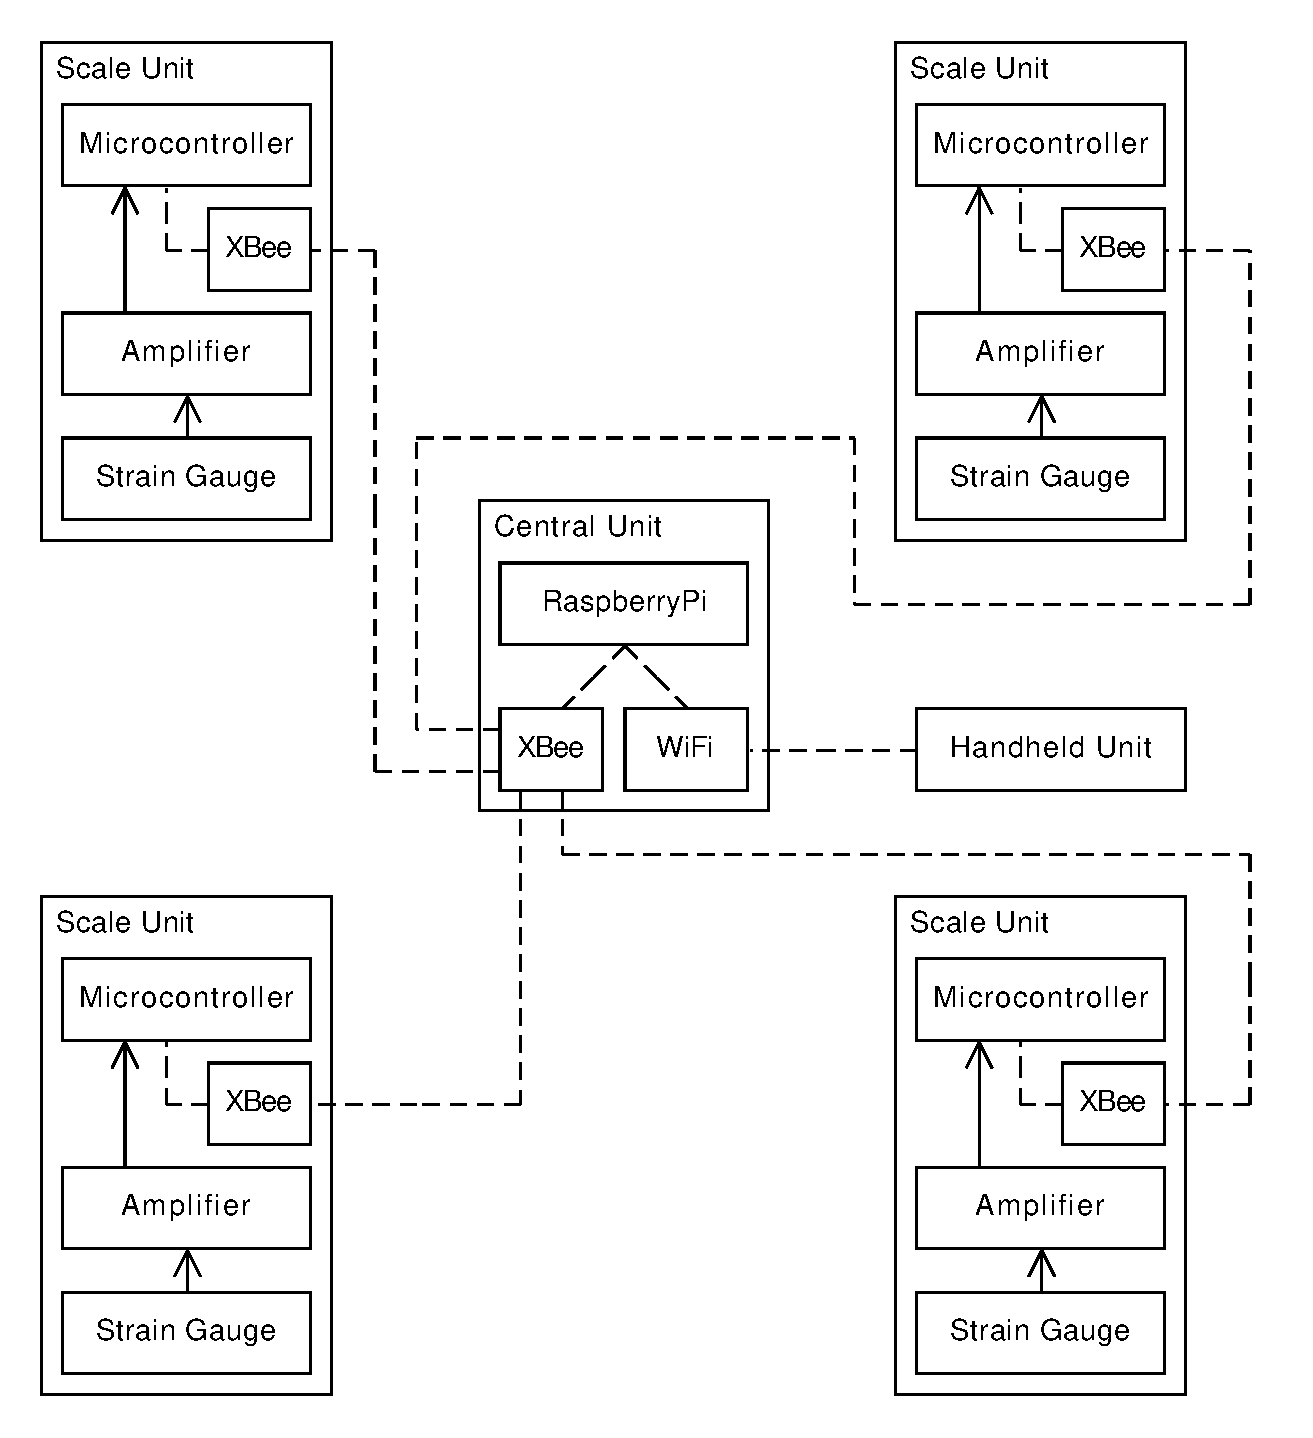
\includegraphics[width=12cm]{figures/block_diagram}
\end{center}
\caption{Block Diagram}
\label{fig:Block Diagram}
\end{figure}

\label{Block Diagram}
\section{Hardware Design}
The proposed solution is to have 4 simple scale units. These units will simply recieve the analogue signal from a loadcell, convert it into a digital form and then send that to a central unit via a wireless communication module. The central unit will recieve messages containing the weight from each of the 4 different scale units. It will then need to provide this information to a user in a standardised way in order to make it accessible from a generic device as required (see sec\ref{section:system}).%TODO 


%%% to be moved to hardware design later.
%This approach of using the central unit to host the information on a network means that any device capable of %connecting to the network and displaying a webpage, will easily be able to manipulat the system and retreive %information. This fits the requirement of being accessible from a generic handheld device such as a phone or %tablet found in ref{section:NFR}.


\section{Software Design}
%TODO introduction to software implementation. C programming language, pthreads, webserver.
The software has been implemented in the C programming language to allow for maximum re-use of components across the master unit (Raspberry Pi, Linux) and the scale units (STM32F4/ARM Cortex M4 microcontroller, no operating system). These Units are connected to each other through a ``star'' network topology using the ZigBee RF modules. One ZigBee, connected to the master unit, is configured as a coordinator (ie. access point) and the four others as routers (or end devices). They join the network with a pre-set network ID and can then communicate wirelessly. To avoid having to store and discover network addresses, only broadcast mode (coordinator to all other devices) and unicast to the coordinator (since the coordinator adress does never change) are used.

%overview
\section{Packet Protocol}
\label{section:software-impl-packets}
ZigBee modules can operate in two seperate communication modes. Firstly, transparent mode is the most basic one, where only very simple packetization (after a time-out or when a buffer is filled) is provided. In this mode it is very simple to set up a basic point-to-point network, but it does not support multiple nodes transmitting at once. In that situation, packets can become interleaved, rendering this mode not very useful for the envisioned star network architecture. Still, it proved useful for initial debugging and manually sending data by connecting the device directly to a serial terminal.

The second mode supported is the ZigBee API, where data is not immediately transmitted, but a series of command packets must be sent to the ZigBee device over the serial connection in order to request data transmission. Here, the ZigBee layer guarantees delivery (up to \textbf{TODO check this number with data sheet and cite} 3 retransmissions) and maintains packet boundaries. The API defines a wrapper packet protocol that is used for sending command and data frames across the serial link\cite[page 35]{xbee-datasheet}.

Originally, a simple packet system was devised to run on top of the transparent mode. In prototyping, this was found to be too unreliable and inefficient due to the aforementioned interleaving of data. Since this design was very similar to the ZigBee API protocol, only few changes were required to send the payload data wrapped in packages conforming to this. The parser was also updated to recognise ``RF data received'' frames and extract the same information from these. This updated protocol is described below:

The payload consists of an \emph{Op-Code} to signify the current operation (ping, pong, measure request, measure response), a \emph{device identifier} that is set at compile-time (through a method call from application to packet layer), and the actual \emph{data} if the packet is a measure response. This data is encoded as ASCII characters representing a hexadecimal number, rather than directly including the bytes. This decision was made to avoid having to escape control characters such as \texttt{0x7E} which defines the beginning of a packet in the ZigBee API. In the original design a \emph{length} byte for the data was included. This was later abandoned since the wrapping API packet already contains a length field from which the data portion's size can be derived.

%TODO define and distinguish packets vs frames.

\begin{figure}
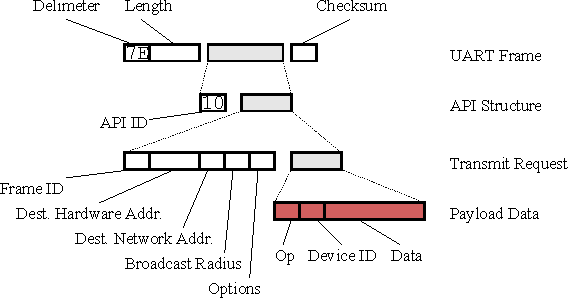
\includegraphics[width=\textwidth]{images/packets.pdf}
\caption{Composition of an example ZigBee API frame transmitted via the UART}
\label{packets-example}
\end{figure}

Besides the data payload described above, the command frames contain a lot of extra information required for parsing the structure. A delimeter marks the beginning of the packet, then two length bytes give the size of the API structure, and a checksum is used for error detection. The API ID specifies the type of frame that is being sent, in this case (\texttt{0x10}) it is a Zigbee Transmit Request frame that includes different target addresses (with special values being used to address the coordinator or broadcast mode). Following these, and a number of extra options that are not used in the context of the project, is the final payload data.

\section{Transport Layer}
The transport layer provides an interface to the serial link (in these implementations, using the UART peripheral of the ARM processors) used to communicate with the ZigBee nodes. This is the main differentiating factor between the master and scale units.

\subsection{Exposed Transport API}
The interface used by higher layers is exposed through \texttt{zb\_transport.h}. It is modelled as a subset of the most basic network operations, only implementing those required by the system -- that is, reading data as individual characters for passing them to the packet layer parser, and writing data as blocks of multiple bytes, for sending complete packets.

First of all, the system must be initialised using \texttt{zb\_transport\_init()}. Then data can be received character by character, in the order received, through the blocking \texttt{zb\_getc()} call. Finally, data can be sent to the device by providing an array of bytes and its size to \texttt{zb\_send()}. The \texttt{zb\_transport\_stop()} method has been added to perform clean-up operations such as closing file handles or freeing dynamically allocated structures on implementations that require it.

\subsection{Linux Implementation}
The Raspberry Pi runs a complete Linux distribution, and the microprocessor's UART peripheral is exposed as a serial port to the system, found in \texttt{/dev/ttyAMA0}. This port can be accessed using standard file operation system calls such as \texttt{read} and \texttt{write} after having been initialised by opening the file and setting a number of standard serial options \cite{posix-serial-programming}. Outside of this software implementation, the system must be configured to not send kernel debug messages to the port\cite{pi-tty}.

A separate thread (implemented using the pthread library \cite{pthread}) is running in the background, continuously monitoring the serial port by blocking on \texttt{read()}. When a character is received on the serial port, it gets stored in a thread safe bounded buffer structure from which characters can later be  retrieved by a higher layer implementation. Thread safety is ensured by using pthread condition variables and locks.

\subsection{Microcontroller Implementation}
On the microcontroller, no threading capabilities besides raw interrupts are available by default, and the serial link is implemented as a peripheral component of the microcontroller. ST provides driver libraries for configuring and accessing such peripherals which have been used extensively for this implementation. Further operating systems such as TinyOS, Kontiki, or InceOS were not initially considered as the team only became aware of their existence well into the implementation phase. However, due to the very simple functionality required of the scale units, their inclusion would likely have made the system more extensible at the cost of complication for the initial implementation.

The UART peripheral provides a small hardware buffer that is currently used as the only buffer in this implementation due to the low frequency of packets and relatively short non-IO bursts in the software. Therefore, the \texttt{zb\_getc} implementation is currently busy-waiting for the memory-mapped UART status register to clear its \emph{RXNE} (Receive buffer non-empty) flag. This is a similiar structure to waiting for a condition variable in a pthread program. %TODO check if we can actually wait for interrupts here to put the processor to sleep, saving power and getting rid of bad busy waiting. Yes we could, but it still wouldn't help the receive-while-sending race condition.

This polling method uses busy waiting, and is therefore is inherently using more power by keeping the processor busy in a loop all the time. It is also less flexible than waiting for interrupts. However, for prototyping and debugging, this made the implementation and testing much easier. It is expected that this part of the system can be re-developed using interrupts and additional software buffering should multi-tasking be required in the future, e.g. if more complicated processing (thus tightening the time constraints) is required.

Since the serial data rate for the ZigBee units (in default configuration) is 9600 baud, and the clock speed of the microcontroller is 168MHz, there is more than enough time to complete any required processing inbetween receiving two characters.

%TODO MATH.

A flaw in the current design is that no data can be received if it is sent while the unit is currently also sending data. This case should be rare, and did not occur during testing, but may still be possible. It should not cause complete system failure, but the packet to be received will be lost and needs to be retransmitted completely by the other end's transport layer, which can currently only be achieved by the application requesting the same packet to be sent again. Retransmission by the ZigBee layer does not solve the issue, as the RF ACK will have been sent, but there is currently no dedicated acknowledgement of UART frames, though this is supported by the ZigBee devices. %TODO reword this - does it make sense?

\section{Packet Layer}
The packet layer provides an abstraction for sending and receiving custom data in a fixed format using the transport layer. Its implementation is identical for all units, the only changes required are in the application layer's initialisation calls.

The first implementation, which was used for testing the transport layer due its simplicity, was based on a custom packet format that had nothing more than the aforementioned data content, a delimeter, and a checksum. The ZigBee units were pre-configured with destination addresses and options, and used in transparent mode.

Due to the issues explained in \ref{section:software-impl-packets}, transparent mode had to be dropped and a second packet layer implementation tailored to the ZigBee API mode was developed using the same API calls. This is described in the following sections. 

\subsection{Packet API}
The public API for the packet layer is defined in \texttt{zb\_packets.h}. 

Initialisation and settings are provided through the \texttt{zb\_packets\_init}, \texttt{zb\_set\_broadcast\_mode}, and \texttt{zb\_set\_device\_id} methods. In the current implementation, broadcast mode is the only way to set the target address: The master unit sends broadcast packages that are received by all scale units, and the scale units send unicast packages targeted only at the master unit. This state is held in a global variable, and it would be trivial to add functionality to support arbitrary target addresses, though this would require for the application layer to know about network or device addresses of the destination.

%TODO missing abstraction: Stop/close/destroy call should be to packets layer and handed down to transport.

\subsection{Parsing Methodology}
The ZigBee API defines data frames transmitted across the serial link between the host and ZigBee device. These packets are parsed and, if the packet is a transmission request, wrapped in a different 802.15.4 packet for transmission over the air, and re-packaged in a serial data frame by the receiving device. The relevant API frames for this design are ''Zigbee Transmit Request'', ``ZigBee Transmission Received'', and ``AT Command Request'' \cite[cf. section 6, API Operation]{xbee-datasheet}.

Re-Transmission if checksums fail or no ACKs are received for these over-the-air packets is handled at the ZigBee layer that is equivalent to the Network layer in the OSI model (\textbf{TODO confirm and cite this}), and in this implementation is completely independent from even the application transport layer.

Parsing of the incoming character stream is achieved through the \texttt{zb\_parse} method which must be called on every character received. It returns a status code to indicate when a complete packet has been received. At this point, globally available variables are filled with the relevant information (op code, device id, data, length) from the packet. The method is implemented as a finite state machine with the state maintained in static local variables. This implementation is inspired by the Yacc parser/lexer architecture\cite{yacc}. In retrospect, these tools could well have been used for the implementation. Due to time constraints in the development phase, and initially starting off with a considerably smaller parser for the simpler packet structure, this was not fully considered before most of the implementation was completed. 

\section{Application Layer}

\begin{figure}
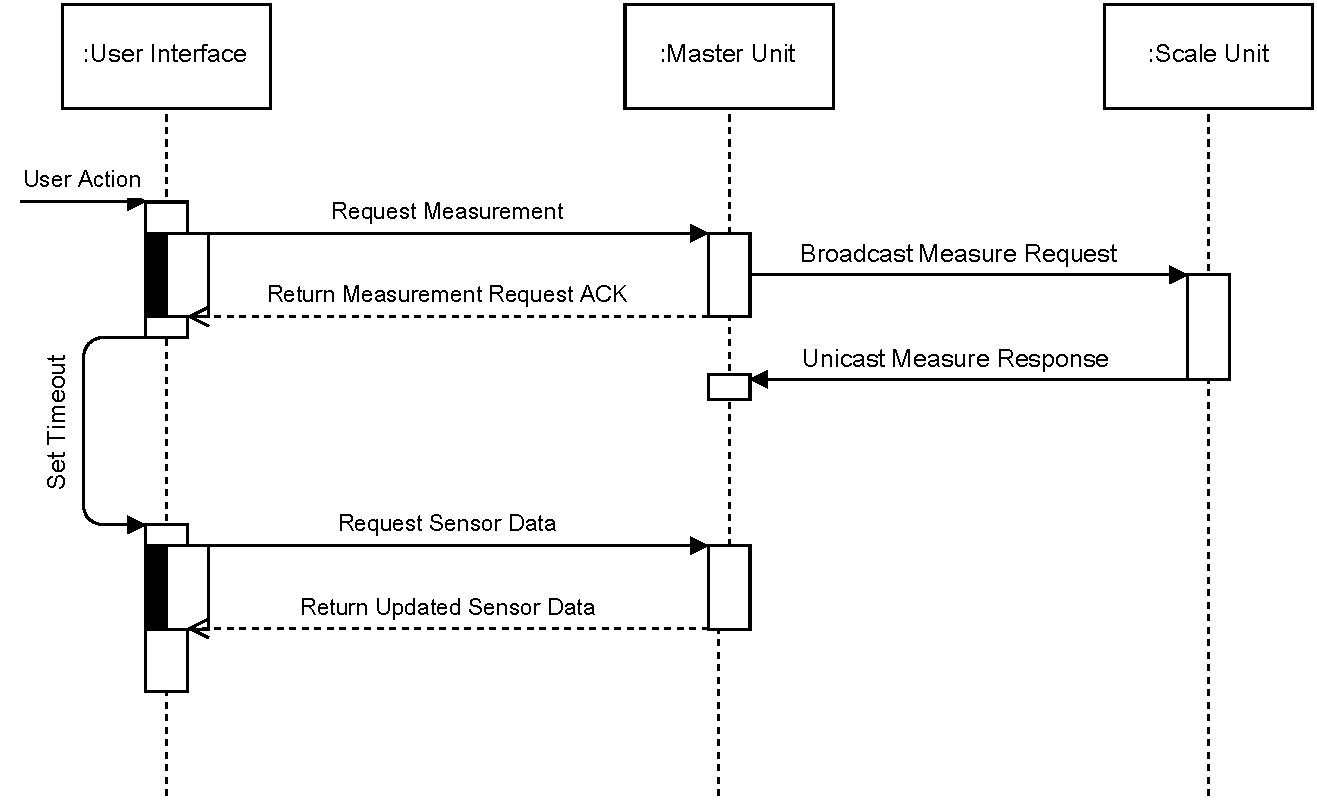
\includegraphics[width=\textwidth]{images/communications-diagram.pdf}
\caption{Application Level Communications Diagram}
\label{communications-diagram}
\end{figure}

Figure \ref{communications-diagram} shows the interaction between the various devices for servicing a user request for updating the measurements. Note that the shown units are entire programs running on different devices, rather than individual threads of control within a single program. One scale unit is shown exemplary. When multiple scale units are used, and all try to respond to the broadcast measure request, their packets are linearised by the receiving ZigBee coordinator.

\subsection{Master Unit}
The master unit program is integrated with a web-server, which is single-threaded to keep the implementation as simple as possible. Since the system will only be used by one or two clients simultaneously, a high-performance implementation is not required as this point. A thread seperate to the webserver uses the packet layer to scan for incoming RF packets and update the thread-safe sensor results data structure with new values as they come in.

Request handlers, which are called when an HTTP request matches an API call path, have been abstracted out into \texttt{requesthandlers.c} so that they can also be invoked manually in the master\_test command-line application. This file manages all state associated with sensors: Their last update time and value, settings such as the calibration offset, as well as a global indicator of when the last RF message was sent. This value is used to provide a primitive time-out mechanism to prevent overloading the serial and RF links if many measure requests come in simultaneously, either due to a bug in the client application or malicious intent. Within one second of the last measurement request, all new incoming measurement or calibration requests are ignored, and an error message is sent to the requesting client.

For serving the user interface, a version of the webserver produced for previous coursework\cite{ns3-coursework} has been used. It was considered to integrate the master unit code with a larger open source software package such as Apache \cite{apache}, possibly as an add-on module. Alternatively, an interface between the request handler C methods and another programming language with existing web-server libraries such as Python could have been developed. However, for prototyping, the decision was made to keep things as simple as possible, and as only a limited amount of time was available, this approach that was already well understood by the team was taken.

The conversion from sensor value to weight is performed on the server. Similarly, the calibration method is implemented by storing an offset for each sensor on the master unit, which is updated with the current sensor readings when the user requests a calibration. As a placeholder for actual calibration and conversion functionality, the conversion is performed by dividing by a constant, where the calibration is just a fixed offset. It is expected that the methods for conversion and calibration will need to be significantly more complicated, as the strain gauge's change in resistance, and thus ADC input voltage, does not scale linearly with weight but can be approximated with \textbf{ASK JOSH WHAT MATHEMATICAL FUCNTION REPERSNTS THIS}.

\subsection{Scale Unit}
The scale unit software has been kept very minimal. The same packet layer implementation written for the master unit is re-used here. The program consists of a single infinite loop that retrieves characters from the UART using the transport layer, calls the parser, and sends a response if a complete valid packet has been retrieved. The response data is read from the Analogue-to-Digital converter (ADC) that is connected to the strain gauge instrumentation amplifier.

The ADC peripheral has been configured in continous conversion DMA (direct memory access) mode. This means that the conversions are handled purely by hardware, and the results can be accessed through a global variable at any time with no additional delay or processing. The conversion rate for this is \textbf{CONVERSION RATE FOR DMA MODE ADC AND SOURCE FOR THIS}.


\subsection{User Interface}
The user interface to the system has been defined in section \ref{requirements} to be a very simple web application that should support taking readings of the current system state by intitiating measurements, as well as providing simple calibration of the scales. A mock-up was drawn up, and based on this a static HTML/CSS prototype was generated. This was then made interactive by attaching Javascript actions to the buttons.

The client side (running in the user's web-browser) logic is implemented using the jQuery Javascript framework \cite{jquery} which provides simple abstractions for modifying the displayed documents (switching between sections and responding to user events such as button clicks), sending asynchronous HTTP requests, and parsing responses to them. This is used to make calls to special paths that are mapped to methods initiating data transfers between the master and scale units, or returning data previously stored on the server:

\begin{itemize}
	\item \texttt{/api/data} returns a JSON \cite{json-spec} object containing the data stored on the master unit for all sensors (raw value, converted value, last response time).
	\item \texttt{/api/calibrate} initiates a measurement on all scale units and sets the values received to be the zero-points for that particular sensor.
	\item \texttt{/api/measure} initiates a measurement and stores the results in a server-side structure to be later retreived by a \texttt{data} request.
\end{itemize}

\begin{figure}
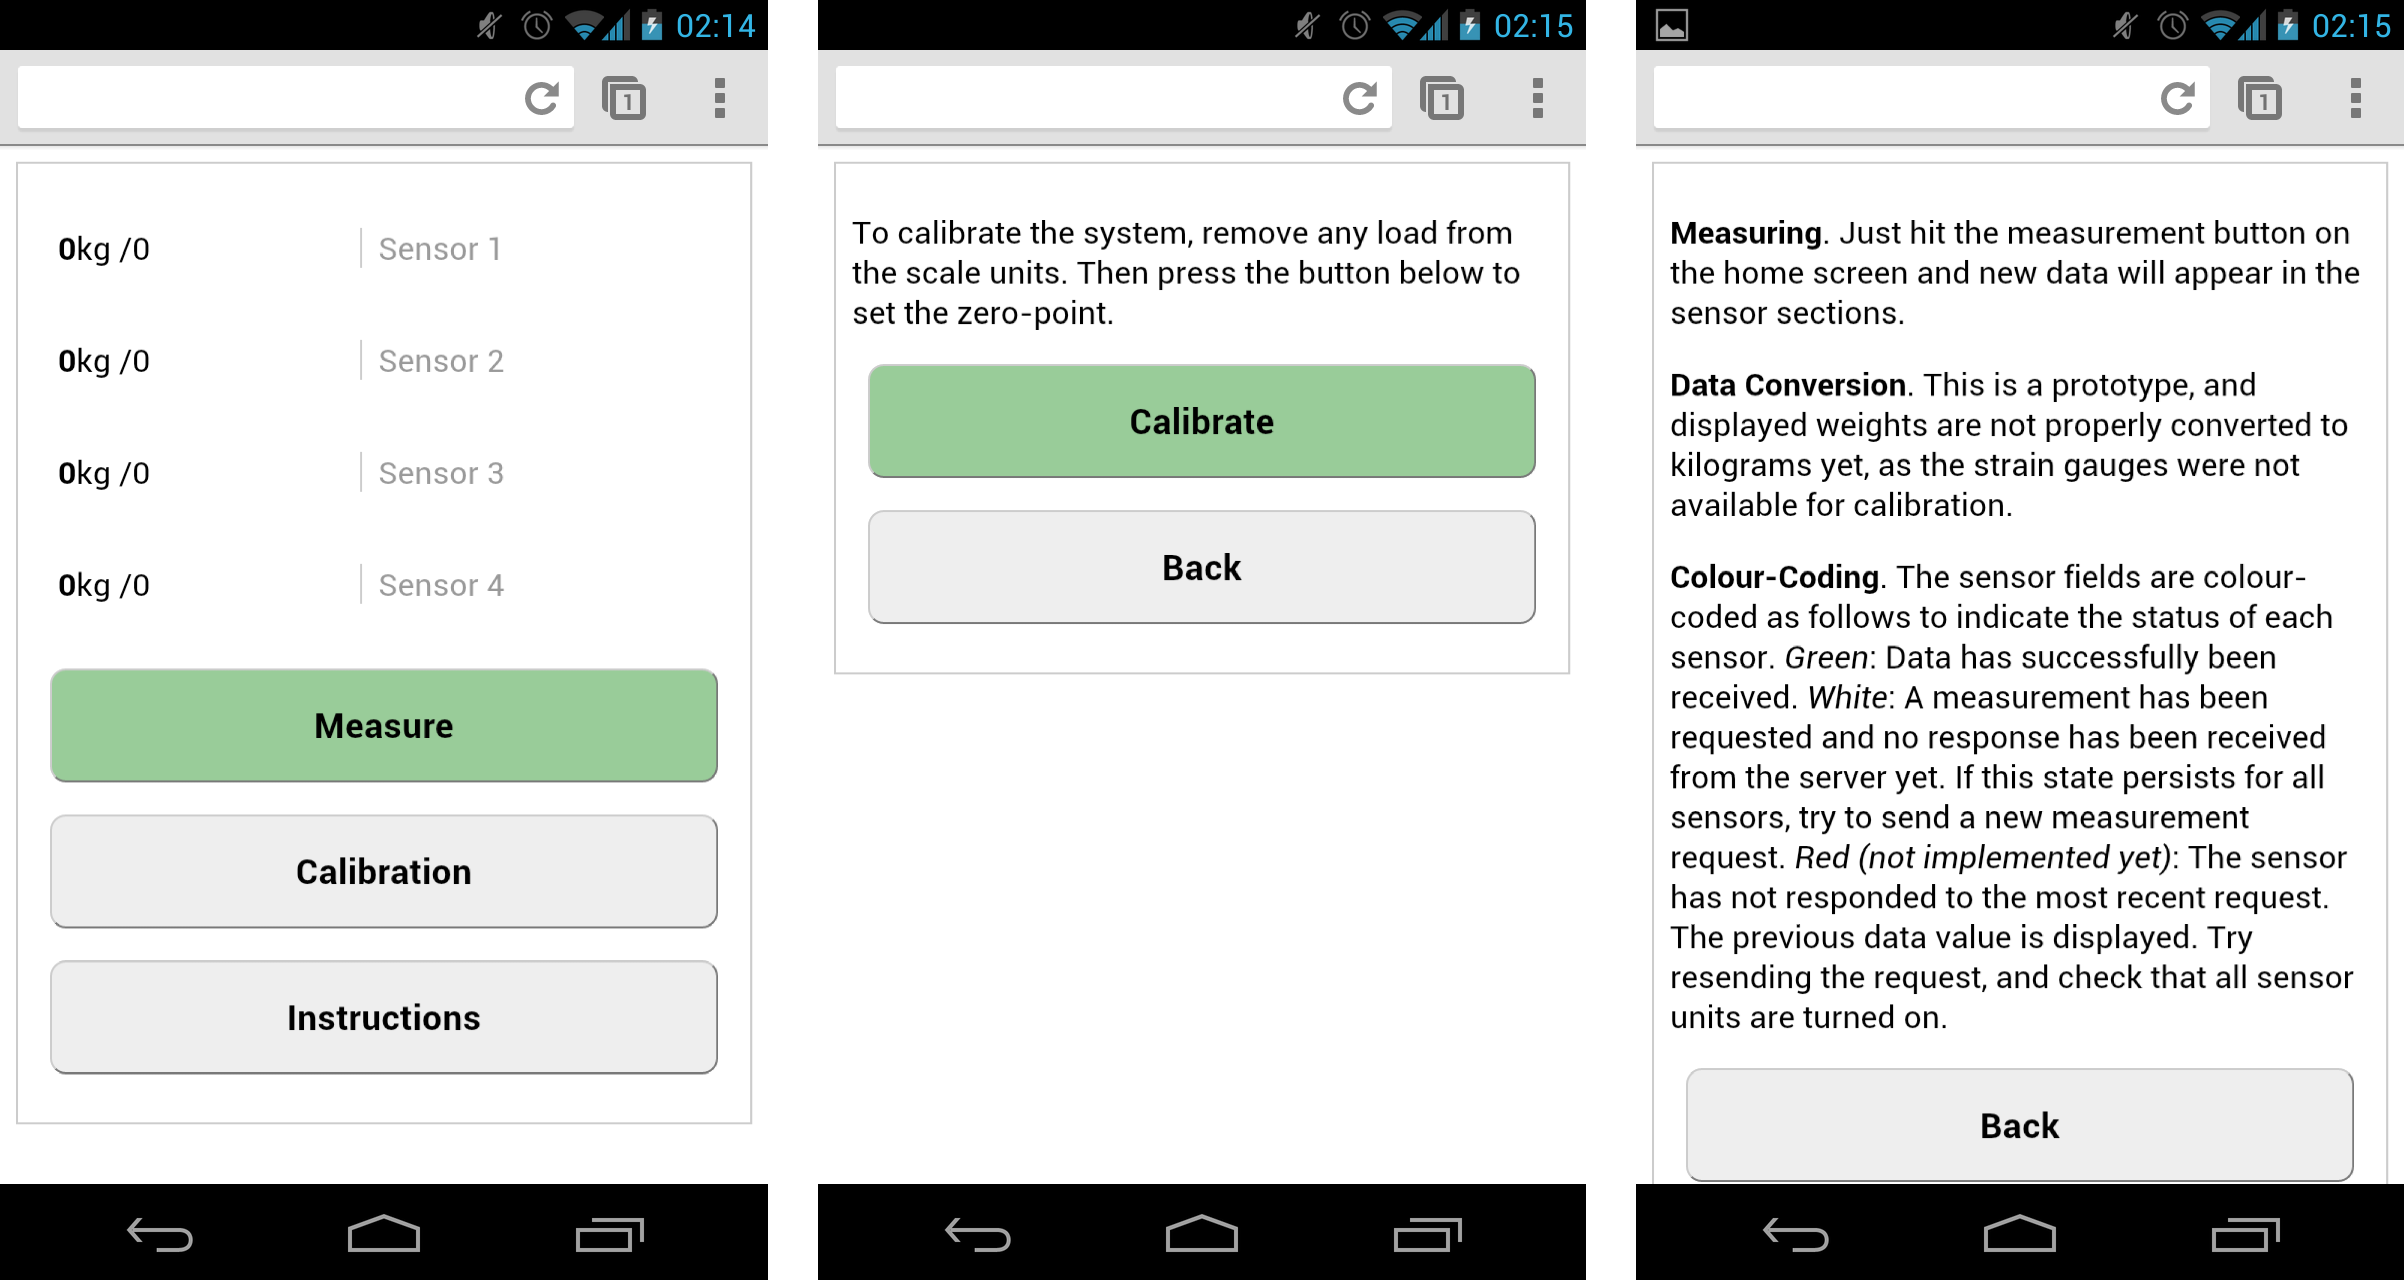
\includegraphics[width=\textwidth]{images/screenshots/ui-screenshot.png}
\caption{User Interface Screens, viewed on an Android phone within the Chrome browser}
\label{ui-screenshot}
\end{figure}

The design was informed by the main target platform which are small touch screens on smart phones (e.g. Android or iOS), or tablets. Therefore, the number of buttons has been kept as low as possible, and the main focus is on displaying crucial information. Colour-coding the background of each sensor section is used to provide visual feedback to user interface actions and system status, to avoid using up more screen real-estate. A quick start guide is included through the ``Instructions'' button. Since calibration can have a very confusing effect if there is still some weights on the scales when it is initiated, this has been made into a two-step process: The user has to open the calibration screen and confirm the action, a helpful note about the effects is displayed with the confirmation button.

Of course, this design leaves room for expansion. For example, one could envision a slider component to view previously retrieved measurements, as well as different display modes to do some data analysis on the raw values received, such as displaying differential weights for the left/right and front/rear distribution. Before final delivery of the system, the scale units must be marked with labels to indicate which wheel they are meant for, and then the ``Sensor n'' labels can be replaced with ``front-left'', and so on.

%==============================================================================
\chapter{Software Implementation}
\label{impl}
%TODO introduction to software implementation. C programming language, pthreads, webserver.
The software has been implemented in the C programming language to allow for maximum re-use of components across the master unit (Raspberry Pi, Linux) and the scale units (STM32F4/ARM Cortex M4 microcontroller, no operating system). These Units are connected to each other through a ``star'' network topology using the ZigBee RF modules. One ZigBee, connected to the master unit, is configured as a coordinator (ie. access point) and the four others as routers (or end devices). They join the network with a pre-set network ID and can then communicate wirelessly. To avoid having to store and discover network addresses, only broadcast mode (coordinator to all other devices) and unicast to the coordinator (since the coordinator adress does never change) are used.

%overview
\section{Packet Protocol}
\label{section:software-impl-packets}
ZigBee modules can operate in two seperate communication modes. Firstly, transparent mode is the most basic one, where only very simple packetization (after a time-out or when a buffer is filled) is provided. In this mode it is very simple to set up a basic point-to-point network, but it does not support multiple nodes transmitting at once. In that situation, packets can become interleaved, rendering this mode not very useful for the envisioned star network architecture. Still, it proved useful for initial debugging and manually sending data by connecting the device directly to a serial terminal.

The second mode supported is the ZigBee API, where data is not immediately transmitted, but a series of command packets must be sent to the ZigBee device over the serial connection in order to request data transmission. Here, the ZigBee layer guarantees delivery (up to \textbf{TODO check this number with data sheet and cite} 3 retransmissions) and maintains packet boundaries. The API defines a wrapper packet protocol that is used for sending command and data frames across the serial link\cite[page 35]{xbee-datasheet}.

Originally, a simple packet system was devised to run on top of the transparent mode. In prototyping, this was found to be too unreliable and inefficient due to the aforementioned interleaving of data. Since this design was very similar to the ZigBee API protocol, only few changes were required to send the payload data wrapped in packages conforming to this. The parser was also updated to recognise ``RF data received'' frames and extract the same information from these. This updated protocol is described below:

The payload consists of an \emph{Op-Code} to signify the current operation (ping, pong, measure request, measure response), a \emph{device identifier} that is set at compile-time (through a method call from application to packet layer), and the actual \emph{data} if the packet is a measure response. This data is encoded as ASCII characters representing a hexadecimal number, rather than directly including the bytes. This decision was made to avoid having to escape control characters such as \texttt{0x7E} which defines the beginning of a packet in the ZigBee API. In the original design a \emph{length} byte for the data was included. This was later abandoned since the wrapping API packet already contains a length field from which the data portion's size can be derived.

%TODO define and distinguish packets vs frames.

\begin{figure}
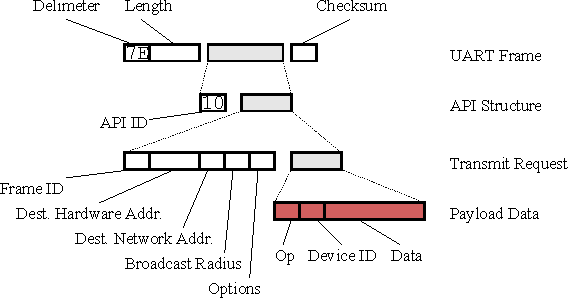
\includegraphics[width=\textwidth]{images/packets.pdf}
\caption{Composition of an example ZigBee API frame transmitted via the UART}
\label{packets-example}
\end{figure}

Besides the data payload described above, the command frames contain a lot of extra information required for parsing the structure. A delimeter marks the beginning of the packet, then two length bytes give the size of the API structure, and a checksum is used for error detection. The API ID specifies the type of frame that is being sent, in this case (\texttt{0x10}) it is a Zigbee Transmit Request frame that includes different target addresses (with special values being used to address the coordinator or broadcast mode). Following these, and a number of extra options that are not used in the context of the project, is the final payload data.

\section{Transport Layer}
The transport layer provides an interface to the serial link (in these implementations, using the UART peripheral of the ARM processors) used to communicate with the ZigBee nodes. This is the main differentiating factor between the master and scale units.

\subsection{Exposed Transport API}
The interface used by higher layers is exposed through \texttt{zb\_transport.h}. It is modelled as a subset of the most basic network operations, only implementing those required by the system -- that is, reading data as individual characters for passing them to the packet layer parser, and writing data as blocks of multiple bytes, for sending complete packets.

First of all, the system must be initialised using \texttt{zb\_transport\_init()}. Then data can be received character by character, in the order received, through the blocking \texttt{zb\_getc()} call. Finally, data can be sent to the device by providing an array of bytes and its size to \texttt{zb\_send()}. The \texttt{zb\_transport\_stop()} method has been added to perform clean-up operations such as closing file handles or freeing dynamically allocated structures on implementations that require it.

\subsection{Linux Implementation}
The Raspberry Pi runs a complete Linux distribution, and the microprocessor's UART peripheral is exposed as a serial port to the system, found in \texttt{/dev/ttyAMA0}. This port can be accessed using standard file operation system calls such as \texttt{read} and \texttt{write} after having been initialised by opening the file and setting a number of standard serial options \cite{posix-serial-programming}. Outside of this software implementation, the system must be configured to not send kernel debug messages to the port\cite{pi-tty}.

A separate thread (implemented using the pthread library \cite{pthread}) is running in the background, continuously monitoring the serial port by blocking on \texttt{read()}. When a character is received on the serial port, it gets stored in a thread safe bounded buffer structure from which characters can later be  retrieved by a higher layer implementation. Thread safety is ensured by using pthread condition variables and locks.

\subsection{Microcontroller Implementation}
On the microcontroller, no threading capabilities besides raw interrupts are available by default, and the serial link is implemented as a peripheral component of the microcontroller. ST provides driver libraries for configuring and accessing such peripherals which have been used extensively for this implementation. Further operating systems such as TinyOS, Kontiki, or InceOS were not initially considered as the team only became aware of their existence well into the implementation phase. However, due to the very simple functionality required of the scale units, their inclusion would likely have made the system more extensible at the cost of complication for the initial implementation.

The UART peripheral provides a small hardware buffer that is currently used as the only buffer in this implementation due to the low frequency of packets and relatively short non-IO bursts in the software. Therefore, the \texttt{zb\_getc} implementation is currently busy-waiting for the memory-mapped UART status register to clear its \emph{RXNE} (Receive buffer non-empty) flag. This is a similiar structure to waiting for a condition variable in a pthread program. %TODO check if we can actually wait for interrupts here to put the processor to sleep, saving power and getting rid of bad busy waiting. Yes we could, but it still wouldn't help the receive-while-sending race condition.

This polling method uses busy waiting, and is therefore is inherently using more power by keeping the processor busy in a loop all the time. It is also less flexible than waiting for interrupts. However, for prototyping and debugging, this made the implementation and testing much easier. It is expected that this part of the system can be re-developed using interrupts and additional software buffering should multi-tasking be required in the future, e.g. if more complicated processing (thus tightening the time constraints) is required.

Since the serial data rate for the ZigBee units (in default configuration) is 9600 baud, and the clock speed of the microcontroller is 168MHz, there is more than enough time to complete any required processing inbetween receiving two characters.

%TODO MATH.

A flaw in the current design is that no data can be received if it is sent while the unit is currently also sending data. This case should be rare, and did not occur during testing, but may still be possible. It should not cause complete system failure, but the packet to be received will be lost and needs to be retransmitted completely by the other end's transport layer, which can currently only be achieved by the application requesting the same packet to be sent again. Retransmission by the ZigBee layer does not solve the issue, as the RF ACK will have been sent, but there is currently no dedicated acknowledgement of UART frames, though this is supported by the ZigBee devices. %TODO reword this - does it make sense?

\section{Packet Layer}
The packet layer provides an abstraction for sending and receiving custom data in a fixed format using the transport layer. Its implementation is identical for all units, the only changes required are in the application layer's initialisation calls.

The first implementation, which was used for testing the transport layer due its simplicity, was based on a custom packet format that had nothing more than the aforementioned data content, a delimeter, and a checksum. The ZigBee units were pre-configured with destination addresses and options, and used in transparent mode.

Due to the issues explained in \ref{section:software-impl-packets}, transparent mode had to be dropped and a second packet layer implementation tailored to the ZigBee API mode was developed using the same API calls. This is described in the following sections. 

\subsection{Packet API}
The public API for the packet layer is defined in \texttt{zb\_packets.h}. 

Initialisation and settings are provided through the \texttt{zb\_packets\_init}, \texttt{zb\_set\_broadcast\_mode}, and \texttt{zb\_set\_device\_id} methods. In the current implementation, broadcast mode is the only way to set the target address: The master unit sends broadcast packages that are received by all scale units, and the scale units send unicast packages targeted only at the master unit. This state is held in a global variable, and it would be trivial to add functionality to support arbitrary target addresses, though this would require for the application layer to know about network or device addresses of the destination.

%TODO missing abstraction: Stop/close/destroy call should be to packets layer and handed down to transport.

\subsection{Parsing Methodology}
The ZigBee API defines data frames transmitted across the serial link between the host and ZigBee device. These packets are parsed and, if the packet is a transmission request, wrapped in a different 802.15.4 packet for transmission over the air, and re-packaged in a serial data frame by the receiving device. The relevant API frames for this design are ''Zigbee Transmit Request'', ``ZigBee Transmission Received'', and ``AT Command Request'' \cite[cf. section 6, API Operation]{xbee-datasheet}.

Re-Transmission if checksums fail or no ACKs are received for these over-the-air packets is handled at the ZigBee layer that is equivalent to the Network layer in the OSI model (\textbf{TODO confirm and cite this}), and in this implementation is completely independent from even the application transport layer.

Parsing of the incoming character stream is achieved through the \texttt{zb\_parse} method which must be called on every character received. It returns a status code to indicate when a complete packet has been received. At this point, globally available variables are filled with the relevant information (op code, device id, data, length) from the packet. The method is implemented as a finite state machine with the state maintained in static local variables. This implementation is inspired by the Yacc parser/lexer architecture\cite{yacc}. In retrospect, these tools could well have been used for the implementation. Due to time constraints in the development phase, and initially starting off with a considerably smaller parser for the simpler packet structure, this was not fully considered before most of the implementation was completed. 

\section{Application Layer}

\begin{figure}
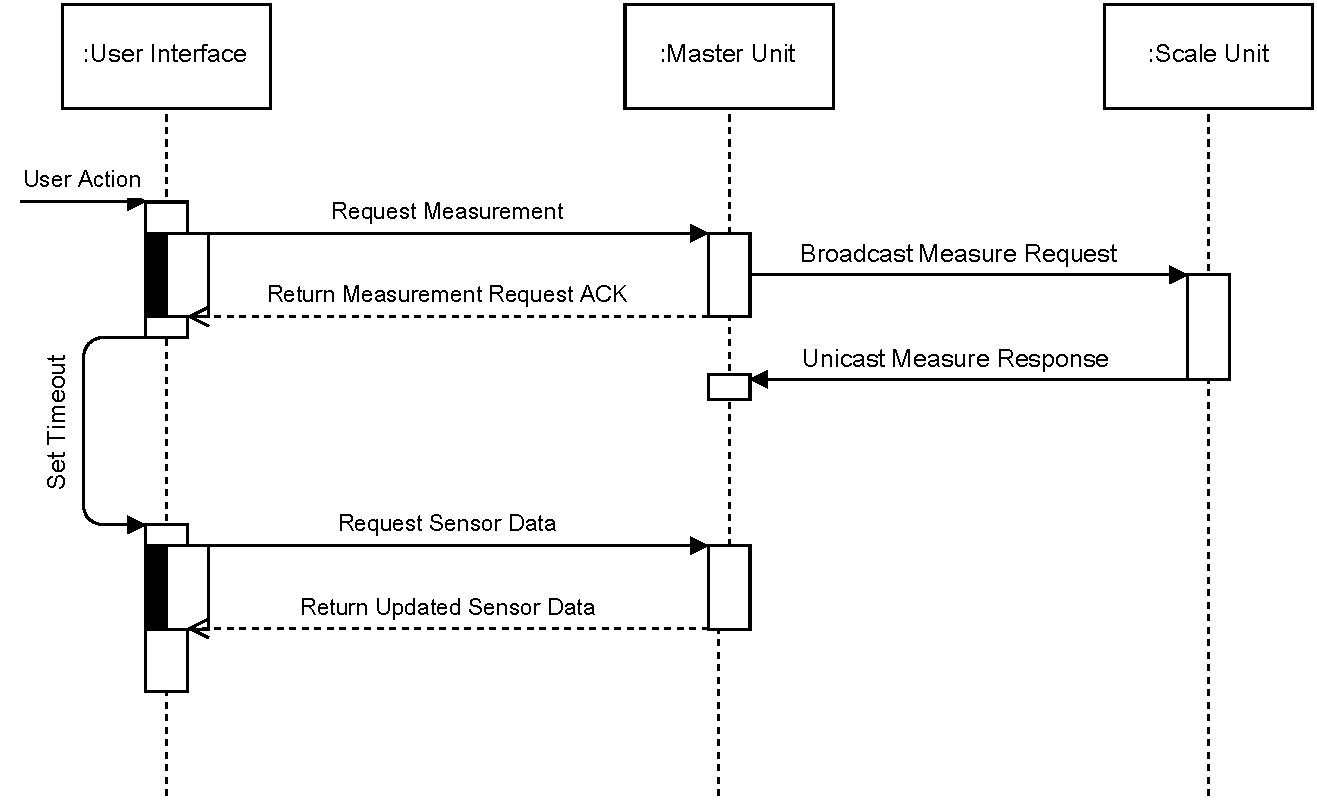
\includegraphics[width=\textwidth]{images/communications-diagram.pdf}
\caption{Application Level Communications Diagram}
\label{communications-diagram}
\end{figure}

Figure \ref{communications-diagram} shows the interaction between the various devices for servicing a user request for updating the measurements. Note that the shown units are entire programs running on different devices, rather than individual threads of control within a single program. One scale unit is shown exemplary. When multiple scale units are used, and all try to respond to the broadcast measure request, their packets are linearised by the receiving ZigBee coordinator.

\subsection{Master Unit}
The master unit program is integrated with a web-server, which is single-threaded to keep the implementation as simple as possible. Since the system will only be used by one or two clients simultaneously, a high-performance implementation is not required as this point. A thread seperate to the webserver uses the packet layer to scan for incoming RF packets and update the thread-safe sensor results data structure with new values as they come in.

Request handlers, which are called when an HTTP request matches an API call path, have been abstracted out into \texttt{requesthandlers.c} so that they can also be invoked manually in the master\_test command-line application. This file manages all state associated with sensors: Their last update time and value, settings such as the calibration offset, as well as a global indicator of when the last RF message was sent. This value is used to provide a primitive time-out mechanism to prevent overloading the serial and RF links if many measure requests come in simultaneously, either due to a bug in the client application or malicious intent. Within one second of the last measurement request, all new incoming measurement or calibration requests are ignored, and an error message is sent to the requesting client.

For serving the user interface, a version of the webserver produced for previous coursework\cite{ns3-coursework} has been used. It was considered to integrate the master unit code with a larger open source software package such as Apache \cite{apache}, possibly as an add-on module. Alternatively, an interface between the request handler C methods and another programming language with existing web-server libraries such as Python could have been developed. However, for prototyping, the decision was made to keep things as simple as possible, and as only a limited amount of time was available, this approach that was already well understood by the team was taken.

The conversion from sensor value to weight is performed on the server. Similarly, the calibration method is implemented by storing an offset for each sensor on the master unit, which is updated with the current sensor readings when the user requests a calibration. As a placeholder for actual calibration and conversion functionality, the conversion is performed by dividing by a constant, where the calibration is just a fixed offset. It is expected that the methods for conversion and calibration will need to be significantly more complicated, as the strain gauge's change in resistance, and thus ADC input voltage, does not scale linearly with weight but can be approximated with \textbf{ASK JOSH WHAT MATHEMATICAL FUCNTION REPERSNTS THIS}.

\subsection{Scale Unit}
The scale unit software has been kept very minimal. The same packet layer implementation written for the master unit is re-used here. The program consists of a single infinite loop that retrieves characters from the UART using the transport layer, calls the parser, and sends a response if a complete valid packet has been retrieved. The response data is read from the Analogue-to-Digital converter (ADC) that is connected to the strain gauge instrumentation amplifier.

The ADC peripheral has been configured in continous conversion DMA (direct memory access) mode. This means that the conversions are handled purely by hardware, and the results can be accessed through a global variable at any time with no additional delay or processing. The conversion rate for this is \textbf{CONVERSION RATE FOR DMA MODE ADC AND SOURCE FOR THIS}.


\subsection{User Interface}
The user interface to the system has been defined in section \ref{requirements} to be a very simple web application that should support taking readings of the current system state by intitiating measurements, as well as providing simple calibration of the scales. A mock-up was drawn up, and based on this a static HTML/CSS prototype was generated. This was then made interactive by attaching Javascript actions to the buttons.

The client side (running in the user's web-browser) logic is implemented using the jQuery Javascript framework \cite{jquery} which provides simple abstractions for modifying the displayed documents (switching between sections and responding to user events such as button clicks), sending asynchronous HTTP requests, and parsing responses to them. This is used to make calls to special paths that are mapped to methods initiating data transfers between the master and scale units, or returning data previously stored on the server:

\begin{itemize}
	\item \texttt{/api/data} returns a JSON \cite{json-spec} object containing the data stored on the master unit for all sensors (raw value, converted value, last response time).
	\item \texttt{/api/calibrate} initiates a measurement on all scale units and sets the values received to be the zero-points for that particular sensor.
	\item \texttt{/api/measure} initiates a measurement and stores the results in a server-side structure to be later retreived by a \texttt{data} request.
\end{itemize}

\begin{figure}
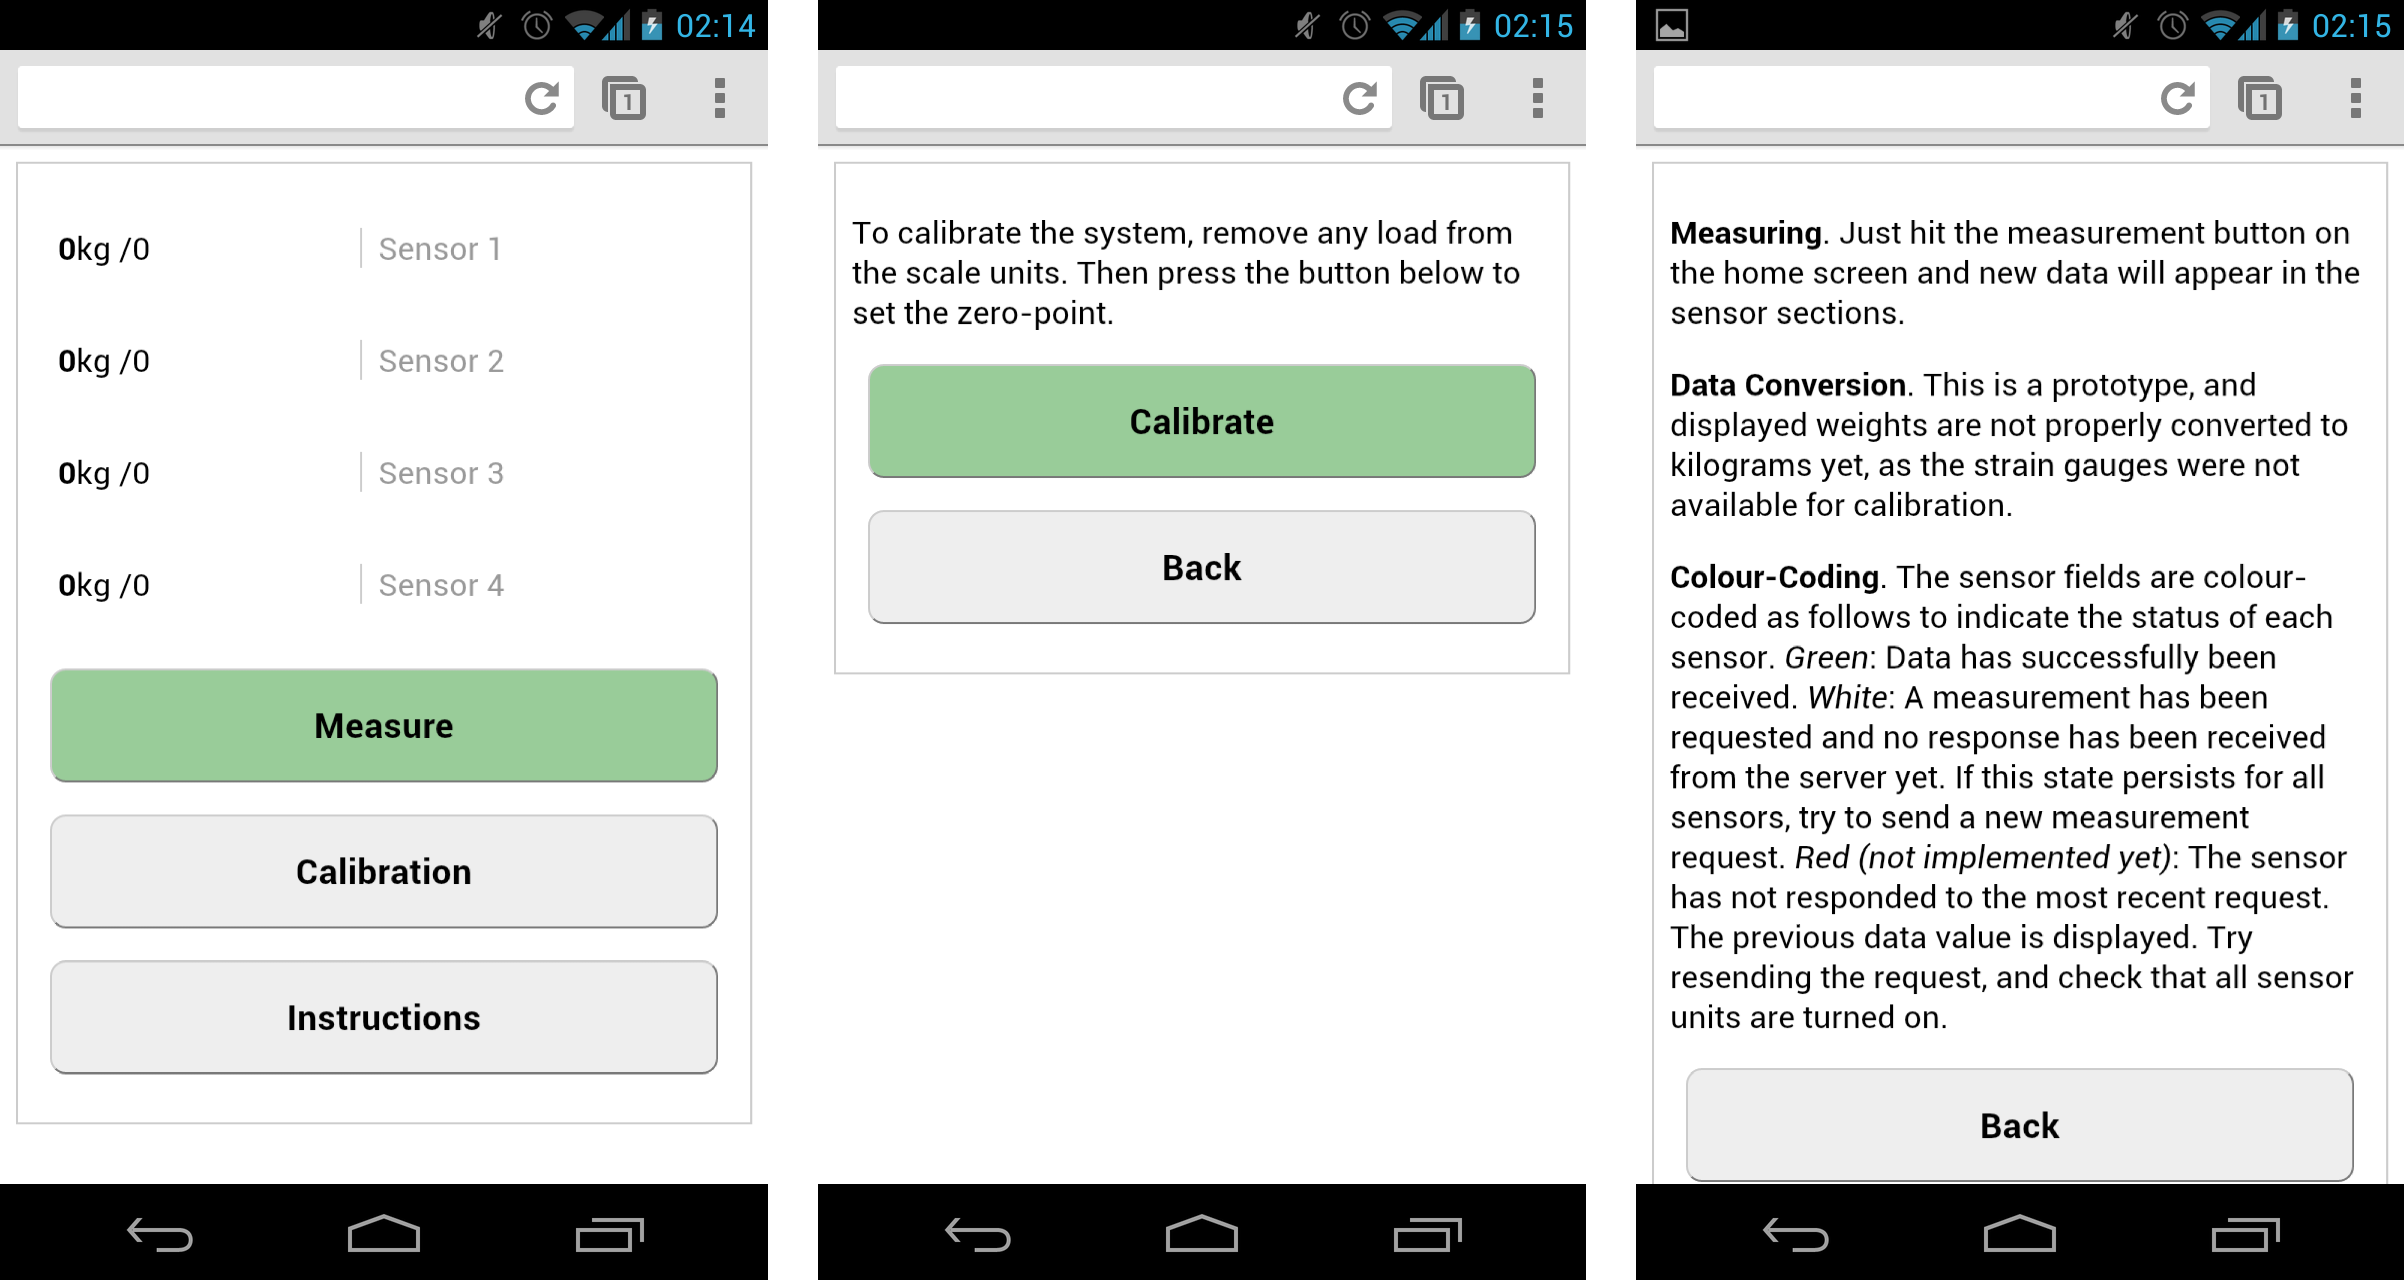
\includegraphics[width=\textwidth]{images/screenshots/ui-screenshot.png}
\caption{User Interface Screens, viewed on an Android phone within the Chrome browser}
\label{ui-screenshot}
\end{figure}

The design was informed by the main target platform which are small touch screens on smart phones (e.g. Android or iOS), or tablets. Therefore, the number of buttons has been kept as low as possible, and the main focus is on displaying crucial information. Colour-coding the background of each sensor section is used to provide visual feedback to user interface actions and system status, to avoid using up more screen real-estate. A quick start guide is included through the ``Instructions'' button. Since calibration can have a very confusing effect if there is still some weights on the scales when it is initiated, this has been made into a two-step process: The user has to open the calibration screen and confirm the action, a helpful note about the effects is displayed with the confirmation button.

Of course, this design leaves room for expansion. For example, one could envision a slider component to view previously retrieved measurements, as well as different display modes to do some data analysis on the raw values received, such as displaying differential weights for the left/right and front/rear distribution. Before final delivery of the system, the scale units must be marked with labels to indicate which wheel they are meant for, and then the ``Sensor n'' labels can be replaced with ``front-left'', and so on.

%==============================================================================
\chapter{Hardware Implementation}
There were a number of different constraints placed on the creation of the initial prototype of the Wireless Weighing System. These constraints come from the PCB construction facilities available at the University of Glasgow. Students are capable of working with the majority of through hole components such as Plastic Dual In-line Packages (PDIP), TO-XX, and some large surface mounted components, this constraint is due to all soldering being done by hand.

Although it is possible to use surface mounted components, there is a high potential in causing damage to the component. With this added risk, the decision was made to only use through hole components, this limited the choice of certain components such as microcontrollers, amplifiers and wireless modules.

Although limited in the number of microcontrollers that are available for use, there is still a few that are available in PDIP packages. However, those that are available are limited in features primarily when it comes to Analogue to Digital Convertors (ADCs). In order to meet the requirements of having a resolution of less than 1kg at least a 10-bit ADC is required, assuming a maximum of 100kg on each scale.

\begin{center}
$N_{ADC} = \frac{V_{in}}{LSB}$
\end{center}
\section{Component Selection}
\subsection{Microcontroller}
The Wireless Weighing System requires two, different microcontrollers, one for the central unit and another for the scale units. Different microcontrollers are being used as the level of performance required from the scale unit system is much lower than that of the central unit.

\subsubsection{The Central Unit}
The central unit requires the ability to access or create a wireless network in order to broadcast data to the display units via an installed web server. The Raspberry Pi \cite{raspberrypi} provides all the functionality that is required, mainly:
	\begin{itemize}
		\item the ability to run the Linux operating system (web server)
		\item Ethernet port
		\item a large number of networking options:
			\begin{itemize} 
				\item USB connectors for potential Bluetooth or WiFi
				\item GPIO pins for RF
				\item UART peripheral, accessible via outside pins
			\end{itemize}
	\end{itemize}
The Raspberry Pi is also ideal as a central unit as it is small and portable, being the size of a credit card. It also has the ability to be connected to a screen and hence provides a platform to both program and debug the system easily. As the Raspberry Pi is powered with a $5\unit{V}$ supply from a USB connection it is possible to have it powered from a computer, wall socket or a battery.

\subsubsection{scale unit}
The microcontroller for the scale unit has much lower requirements than the controller required for the central unit. The primary requirement for the scale units is the ability to take data from the strain gauges, this requires an Analogue to Digital Converter (ADC) to convert the analogue signal from the load cell into a digital signal that can be read by the microcontroller. Most microcontroller packages contain an ADC, so finding a package which would meet the requirements without the addition of an larger external ADC became a primary aim of the team in the selection of a microcontroller for the scale units. 

\centerline{\(\frac{V_{FS}}{2^{N}} = LSB  \) \cite{edp2}}
\label{LSBeq}

Equation ~\ref{LSBeq} is normally used to show the Least Significant Bit, or the change in input voltage required to change the output by exactly 1 bit. This equation can, however, be changed to show the change in weight to change the output by exactly 1 bit.
The requirements state that the full weight that the system is required to measure will be a maximum of 250kg. Although each scale will not have to take the full weight of car, the weight distribution is unknown, therefore, the design decision was made to ensure that each scale would be rated to 250kg.  \\

\centerline{$\frac{Full Weight}{2^{N}} = LSB$}  \label{LSBeq2}

The HCS08 family of microcontrollers from Freescale would have been the first choice for the scale units due to the team's familiarity to the architecture from previous electronics courses. However, the HCS08 \cite{HCS08} PDIP components only have a 10 bit ADC.\\

\centerline{$\frac{250kg}{2^{10}} = 0.24kg$} \label{LSBeq3}

Although this meets the client's requirements and the MC9S08GB60 \cite{MC9S08GB60} comes in an SDIP package, if a 12-bit ADC was used the accuracy of the scale units would be greatly increased. Whilst consulting Dr Martin Macauley about which microcontrollers could be used by the development tools already available in the School of Electronics and Electrical Engineering, the STM32Fx Discovery series of microcontroller boards was mentioned. The STM32F4 Discovery \cite{STM32F4} boards come pre-assembled, and in addition to the microcontroller include a programmer and USB debugging interface, as well as a hardware UART unit for serial communication. The ARM Cortex M4 processor used also comes with a 12-bit ADC. This will make development simpler than designing a complete circuit around a discrete microcontroller unit.  Using a 12-bit ADC will allow a resolution from the strain gauge of less than 100g. 
\\

\centerline{$\frac{250kg}{2^{12}} = 0.06kg$}

However, if the system were to be mass-produced, it would certainly be more economical to manufacture purpose built PCBs that include the microprocessor and only the required peripheral components. 

\subsection{Wireless Communication Modules}
One of the primary requirements from UGRacing was that the devices were 'wireless' for both ease of use but also to reduce the number of trip hazards in the workshop. There are a number of different options for wireless communications.
\subsubsection{RF Transceiver}
Wireless communication in one of the simplest forms is with two RF Transceivers. Although initially looked at due to the cost effectiveness of using RF Transceivers, it was decided that having to create a wireless communication protocol would both complicate the creation of the Wireless Weighing System unnecessarily.
\subsubsection{Bluetooth}
Bluetooth is a wireless communication protocol which extends a serial port. Bluetooth 1.0 however, is designed for simple point-to-point communication. However, the Wireless Weighing System requires a total of five units meaning the use of Bluetooth 1.0 would require connections to be broken and reconnected every time a measurement is taken.  Bluetooth 2.0 is however, capable of having a multipoint network topology with a single Master Unit and multiple Slaves. Bluetooth devices do not come in packages which can be easily integrated into systems without the addition of breakout boards. Bluetooth 2.0 also requires a large amount of setup in order to create the wireless network required by the Wireless Weighing System.
\subsubsection{ZigBee}
Much like Bluetooth, the ZigBee communication devices are used to extend serial ports. Series 1 (802.15.04) just like Bluetooth 1.0 is only capable of point-to-point communication, and Series 2 can be used to create both simple but also much more complex networks. The ZigBee devices come in a through hole package, and set up for microcontrollers is both simpler than for Bluetooth and has been well documented by the enthusiast community. Due to this the ZigBee Series 2 was chosen as the preferred wireless communication module for the system.

\subsection{Strain Gauge and Wheatstone Bridge}
\begin{figure}
\begin{center}
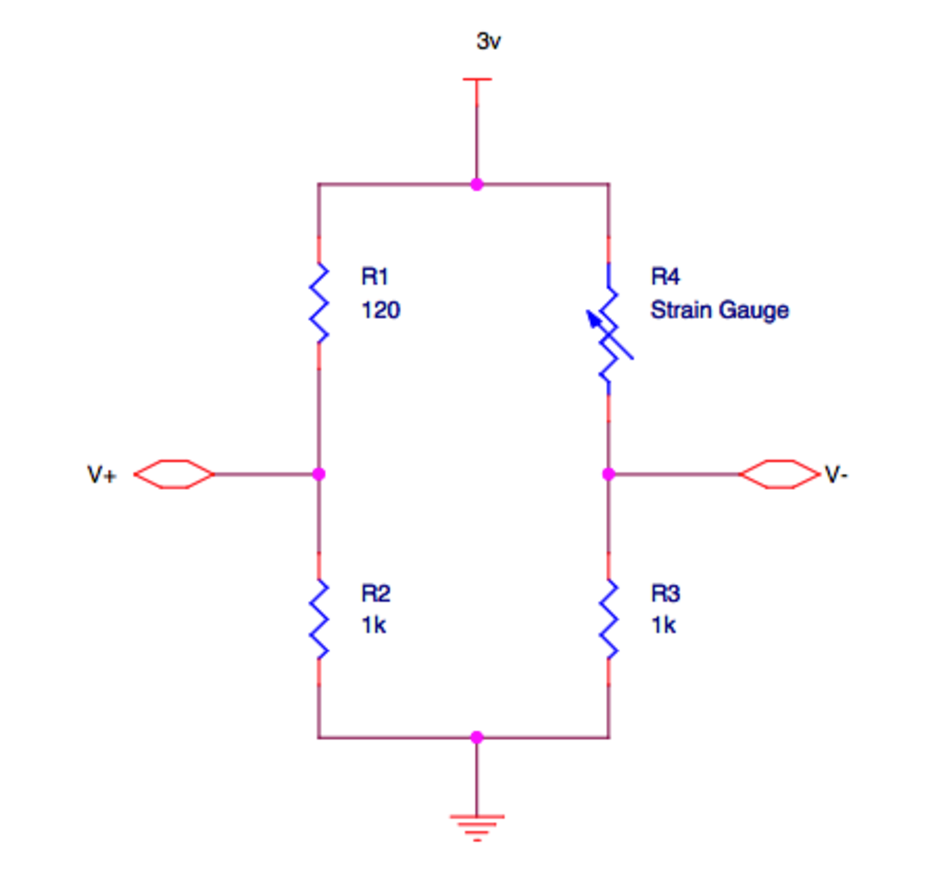
\includegraphics[width=8cm]{implementation/figures/bridge_diagram}
\end{center}
\caption{Bridge Diagram}
\label{fig:Bridge Diagram}
\end{figure}

A strain gauge is a component that changes its resistance value based on how stretched or compressed it is, it is therefore good for use in measuring strain which can in turn be used to calculate the weight of an object e.g. a car. When the client UGR commissioned the product they had already selected a strain gauge for use in the system this would be attached to a machanical device creating a load cell, in particular the N11-MA-5-120-11 mild steel foil strain gauge. The relevant specifications of this are that it is $5mm$ long, it has a gauge factor of $2.1$ and has a base resistance of $120\Omega$.

If a strain gauge changes resistance based on the force exerted on it, one can determin how much force by applying a voltage across the gauge and appreciating the changing behaviour of the circuit. To fully explain the relationship between force applied and resistance the datasheet of the gauge was consulted, which revealed the equation.


\centerline{$K \times \frac{\Delta L}{L} = \frac{\Delta R}{R}$}

 (where L is length of the device, K is the gauge factor and R is the resistance).  

The datasheet also recommends using a wheatstone bridge configeration on the output of the gauge as seen in figure ~\ref{fig:Bridge Diagram}. This configuration allows the output voltage to be $0$ when there is no force applied and using the right arm as one might use a control group in an experiment it allows for obvious observation of change. This change in resistance is normally tiny most gauges having a maximum $\Delta$L of between $2\%$ and $4\%$, this being the case the maximum output voltage from the wheatstone bridge is also small and therefore requires an instrumentation amplifier. This instrumentation amplifier helps to bring the voltage difference on the output to a manageable level for the microcontroller so that small changes in resistance can have a bigger and therefore more noticeable change in voltage. 

The wheatstone bridge is a simple system relying on the principle of voltage dividers and therefore rely on the equation:

\centerline{$V_{out} = V_{in} \times \frac{R2}{R_{total}}$}

When looking at fig ~\ref{fig:Bridge Diagram} we can see that when there is no force applied the voltage across the output will be $0$ as the voltages at both point $V_-$ and $V_+$ will be $3 \times \frac{1000}{1120}$ which is equal to $2.68V$. Now if instead there were a force applied to the strain gauge changing its resistance by 10$\Omega$ then the voltage at point $V_-$ would be $3 \times \frac{1000}{1130}$, which is equal to $2.65V$ and at point $V_+$ it would still be at $2.68V$. therefore the output voltage would be the difference between these two voltages i.e. $0.03V$. The voltage at both points is fed to an instrumentation amplifier, which then magnifies the voltage difference to a more substantial level for the microcontroller to process. 

Given that the client is creating their own load cells that have not started the production process yet it is impossible to say what the maximum strain applied to the strain gauge might be. This being the case calculating the required gain of the instrumentation amplifier is also impossible, the decision has therefore been made to model a strain gauge using a simple potentiometer. This allows us to prototype the load cell, enabeling the testing and demonstation of the system, once the load cell is completed it is a simple calculation to find the required gain for the instrumentation amplifier. 

Using a potentiometer that has resistance between $0\Omega$ and $1000\Omega$ and a resistor in parallel of $430\Omega$ a model was made to simulat a load cell. Using the parallel restistor equation we see that the resistance varies between $0$ and $\frac{430 \times 1000}{430 + 1000}$  which equals $300\Omega$. As we know that the strain gauge is at least $120\Omega$, the lowest resistance that the potentiometer should be reduced to is $166\Omega$ as this gives a total $120\Omega$ when in parallel with $430\Omega$ static resistor. Using the equations stated previously this means that the output voltage varies between $0V$ and $0.37V$. This model is obviously not perfect as the real strain gauge should only be varying in the milliohm range and the voltage would also therefore be varying in more like millivolts, but it suits the purpose of showing that the communication system works. 
\subsection{Instrumentation Amplifier}
\label{ina}
The client suggested an amplifier for the project at the start, this being the INA129. This is an amplifier requireing little power, that is accurate and requires only $700\mu$ quiescent current and therefore meets the requirements of the scale units fairly well.

As stated an Instrumentation amplifier is required to increase the range of output voltage from the wheatstone bridge to a more manageable level for the microcontroller. Given that a microcontroller that has a $3$ volt ADC is being used, the best thing to do is amplify the largest possible output from the bridge up to $3$ volts that way the output should range from $0$ to $3$ volts. 

Given that the maximum voltage on the output of the wheatstone bridge is $0.37V$ this would make the required gain of the INA $\frac{3V}{0.37V}$ which is $8.10V$. So using the equation for gain obtained from the datasheet of the INA: \(Gain(A_{v}) = \frac{V_{out}}{V_{in}}\) and the equation to calibrate the INA for this amplification: 
$A_v = 1 + \frac{2R_a}{R_g}$ therefore in this case $A_v = 1 + \frac{49.4K}{8.1}$

Manipulating this equation you find that $R_g = \frac{2R_a}{A_v - 1}$ plugging in the desired gain of $8.1$ and the value for $R_a$ defined by the data sheet for the INA it can be shown that $R_g$ should be a $7.0K\Omega$ resistor. 
\subsection{Power}
Given that the scale units are required to be wireless, there is a necessity to use some form of battery power in order to keep them running. The client also requested that the batteries be easily replaceable i.e. available in most stores that sell batteries. This being the case there were certain limitations on choice for battery power. 

On each scale unit there is a 5 volt regulator, this is in order to stop any power source providing more than 5 volts from damage the microcontroller; this device will draw a large amount of current if the power source is providing a voltage that is significantly more than 5 volts. This was also a serious consideration when making a decision on power source.

Several options were initially considered such as a 9V lithium battery, but it was decided that this would have too much power drained by the voltage regulator as power dissipated is: $(V_{in} - V_{out}) times I_out$
\section{PCB Design}
\label{pcb}
OrCAD Capture from Cadence in conjunction with PCB Editor from Allegro was used to create the schematic and PCB respectively.  An additional component library was required to allow simulation in OrCAD Capture and placement in PCB Editor. The following components were created by Ian Young (Department of Electronic and Electrical Engineering) specifically for use in this project:
	\begin{itemize}
		\item Digi International XBee S2 module
		\item $13\times2$ Header for connecting the Raspberry Pi
		\item STM32F4 breakout connectors
	\end{itemize}

\subsection{Central Unit}
\begin{figure}
\begin{center}
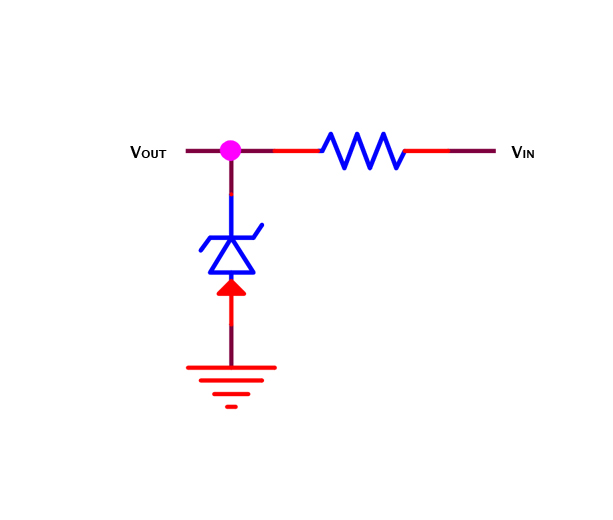
\includegraphics[width=8cm]{implementation/figures/GPIOprotection}
\end{center}
\caption{GPIO Pin Protection}
\label{fig:GPIOprotection}
\end{figure}


The Central Unit is controlled by a Raspberry Pi, and therefore the PCB for holding the ZigBee module is required to connect to the GPIO headers Raspberry Pi.  Initially it was thought that this could be done directly, however on further inspection it was discovered that the Raspberry Pi is very sensitive to signals above \(50mA\) at \(3.3v\). It was decided to make a protection circuit for each of the GPIO pins that were in use. 

A simple protection circuit can be created using a resistor and Zener diode as seen in \textbf{Figure \ref{fig:GPIOprotection}}.  Zener diodes are much like other types of diodes in that it allows current to flow freely in one direction, however unlike other diodes if the voltage is above the 'breakdown' voltage it is allowed to flow as well. Using this property of Zener diodes a simple DC voltage regulator can be created when placed in series with a resistor, if the voltage coming into the system, \(V_{IN}\), is greater than the breakdown voltage of the Zener diode it flows to ground rather than to the GPIO pin. Therefore, a \(3v3\) Zener diode was used with a \(330\Omega\) resistor. The resistor limits the current that goes into the Zener diode, protecting the overall circuit.

Due to the fact that the Raspberry Pi can only produce $50mA$ over the $3v3$ pin, in order to power the XBee module that uses over close to $50mA$ when broadcasting, the $5v$ pin on the Raspberry Pi was need. This can provide up to $700mA$ although at $5v$, this meant that a $3v3$ voltage regulator was required to power the XBee module, this came in the form of an 'ST LD1117' which was available from the University of Glasgow Electrical Components Store. The 'ST LD1117' comes with a low drop out voltage of $1v$ therefore requiring a minimum supply of $4v$. With the voltage regulator come the decoupling capacitors, as suggested by the supplied datasheet.

The pins between the Raspberry Pi and XBee module were connected as shown in Figure ~\ref{Pi2XBeeTable}.

\label{Pi2XBeeTable}
\begin{center}
  \begin{tabular}{| l | l | l | l |}
    \hline
    \bf{Pin (Rapsberry Pi)} & \bf{Function (Rapsberry Pi)} & \bf{Pin (XBee)} & \bf{Function (XBee)} \\ \hline
     - & - & 1 & \(V_{CC}\) \\ \hline
	10 & \(Rx\) & 2 & \(D_{OUT}\) \\ \hline
	8 & \(Tx\) & 3 & \(D_{IN}\) \\ \hline
	12 & \(GPIO\) & 5 & \(Reset\) \\ \hline
	25 & \(GND\) & 10 & \(GND\) \\ \hline
	13 & \(GPIO\) & 12 & \(Sleep\) \\ \hline
	11 & \(GPIO\) & 13 & \(CTS\) \\ \hline
	7 & \(GPIO\) & 16 & \(RTS\) \\
    \hline
  \end{tabular}
\end{center}

In addition to the pins required by the XBee module, three LEDs were placed on the Central Unit PCB. One LED is connected directly to the power supply showing that the board has power, the other two are connected to GPIO pins to be used for any purpose necessary.

As the Central Unit does not require a wireless power supply, using the standard USB power cable was acceptable and provides a constant $5v$, $1000mA$ supply.

\subsection{Scale Unit}
The Scale Unit is controlled by an STM32Fx Discovery series microcontroller, much like for the Central Unit a simple PCB is required to interface the XBee modules to the controller.  Unlike the Central Unit however, protection circuits are not required, instead the Scale Units requires a mobile power supply to allow a completely wireless system.

In order to keep the system as simple as possible it was decided to use a single 5v voltage regulator connected to the STM32Fx Discovery board. The STM32Fx Discovery has a 5v rail which can be used as a 5v supply when connected to USB power, or as an input if the USB cable is not connected. As well as the 5v rail the STM32Fx Discovery board also provides a regulated 3v supply, via either the $V_{DD}$ or 3v pins. This supply will be used for power the XBee modules which have a supply voltage range of 2.8v-3.4v as well as any other circuitry required for the analogue design.

The analogue as designed in section >< was placed close together on the PCB keeping it away from the digital data tracks in order to reduce interference.

The initial design integrated PCB headers to directly interface with all the STM32F4 Discovery pins, however for the initial prototype three headers were used instead; two 6-pin headers, and one 16-pin header. Instead of having a singular power supply option, it was decided to instead create an interface to allow a number of different power supply options. This was implemented with a simple 2-pin molex header, which allows the board to be connected with a lab power pack and batteries simply by changing the connector. In addition to the power supply header a jumper was placed on the power tracks to measure the current being used by the system to allow accurate power usage to be calculated.

\begin{center}
  \begin{tabular}{| l | l | l | l | l |}
    \hline
    \bf{Pin (ARM)} & \bf{Function (ARM)} & \bf{Pin (XBee)} & \bf{Function (XBee)}  & \bf{Other}\\ \hline
         $V_{DD}$ & $3v $& $1 $& $V_{CC} $& $ - $\\ \hline
	 $PD9$ & \(Rx\) &$ 2$ &$ D_{OUT}$ &$ - $\\ \hline
	 $PD8 $& \(Tx\) &$ 3$ &$ D_{IN}$ & $- $\\ \hline
	 $PD12$ & \(RTS\) & $5$ & $CTS$ &$ - $ \\ \hline
	 $PD11$ & $CTS$ & $16$ & $RTS$ & $-$ \\ \hline
	 $GND$ & \(GND\) & $10$ & \(GND\) & $-$\\ \hline
	$PC2 $ & \(GPIO\) & 12 & \(Sleep\) & $-$\\ \hline
	$PC3 $ & \(GPIO\) & 10 & \(Reset\) & $-$ \\
    \hline
  \end{tabular}
\label{interfaceARMXBee}\\
Figure ~\ref{interfaceARMXBee}: Connection between ARM and XBee units
\end{center}
%==============================================================================
\chapter{Evaluation}
This section outlines how the system was evaluated and the results of that evaluation.

\subsection{Testing Strategy and Results}

In order to test the system fully there is a requirement to interface with the yet unbuilt load cell units, which is of course not currently possible. On the otherhand it has been possible to test to a reasonable degree the level of accuracy of the system using the potentionmeter based model of the load cell, this is done by repeatedly requesting measurements from the scale units without changing the resistance levels and detecting the variance on the output. 

RESULTS THAT WE HAVNT DONE YET EEEEK?

Output current tests
//TODO


\subsection{Status Report}

Analogue Design tested by replacing strain gauge with potentiometer of same resistance range, but it still does not work with the calculated gain resistance for the differential amplifier.

\subsection{Future Work}

If the project were to have more time dedicated to it, it would be prudent to test the ability of the system to deal with interference in both its ability to handle any packet loss or corruption but also the level of interference needed to cause packet corruption. If it were found that the packets were easily corrupted or that the system does not handle packet loss in an appropriate manner it might also be prudent to find a solution to this problem.

Integrate the Raspberry Pi master unit with a USB wifi dongle, configure hostapd and dnsmasq to create a hot-spot without hte need for an external router.

Of course given that currently the system does not correctly interface to the load cells, future work would almost certainly require modifications to the analogue design especially the instrumentation amplifier's calibration. It would then be highly important to test the accuracy of the system using known weights and noting the output of the system. After this testing process further calibration would almost certainly be required potentially in both software tools and analogue design. 

Scale units should be ported to M0 based system which will lead to smaller PCB. Need to be placed in IP-65 boxes to meet client's requirements.
WHAT IS MO BASED?

Certain simple but inefficient solutions were given to problems that could be increased in complexity in order to reduce power usage, such as the ZigBee units configuration as router devices. This was done in order to stop them from going into "sleep" mode as they would do whilst configured as end-devices, stopping them from recieving new instruction without further coding. It would also be possible to implement some sort of transport layer logic in order to support pin sleep mode which would turn the radio off when not required.

Currently there is no feedback from the user interface if the unit is unresponsive to a measurement request, this could easy be corrected if future work were to be performed on the system. 

Run a user test with mechanical engineers who will be using the system, and confirm that it is simple enough for them to set-up and take down for redeployment in different locations. Provide a user manual.
%==============================================================================
\chapter{Conclusion}

A great project!

%==============================================================================
\section{Contributions}

Here we explain that Lewis Carroll wrote chapter \ref{intro}. John Wayne
was out riding his horse every day and didn't do anything. Marilyn Monroe
was great at getting the requirements specification and coordinating the
writing of the report. Betty Davis did the coding of the kernel of the
project, described in Chapter \ref{impl}.  James Dean handled the
multimedia content of the project.

%==============================================================================
\bibliographystyle{plain}
\bibliography{TeamN}
\newpage
\appendix
\chapter{Schematics}
\chapter{PCB Photomask}
\begin{figure}[H]
\begin{center}
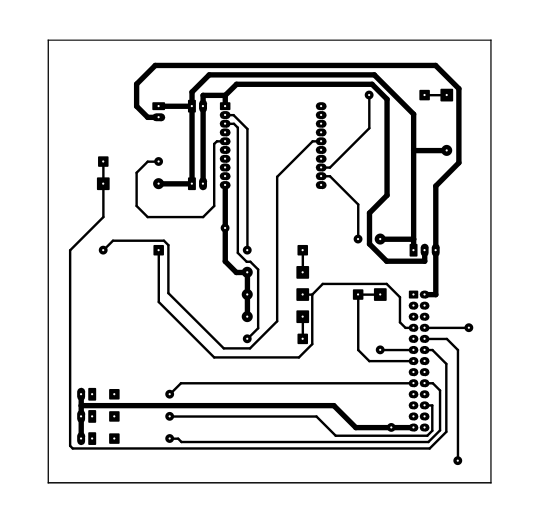
\includegraphics{figures/Pi2XBee_bottom}
\end{center}
\caption{PCB Photomask: RaspberryPi to XBee - Bottom}
\label{fig:Pi2XBee2}
\end{figure}

\begin{figure}[H]
\begin{center}
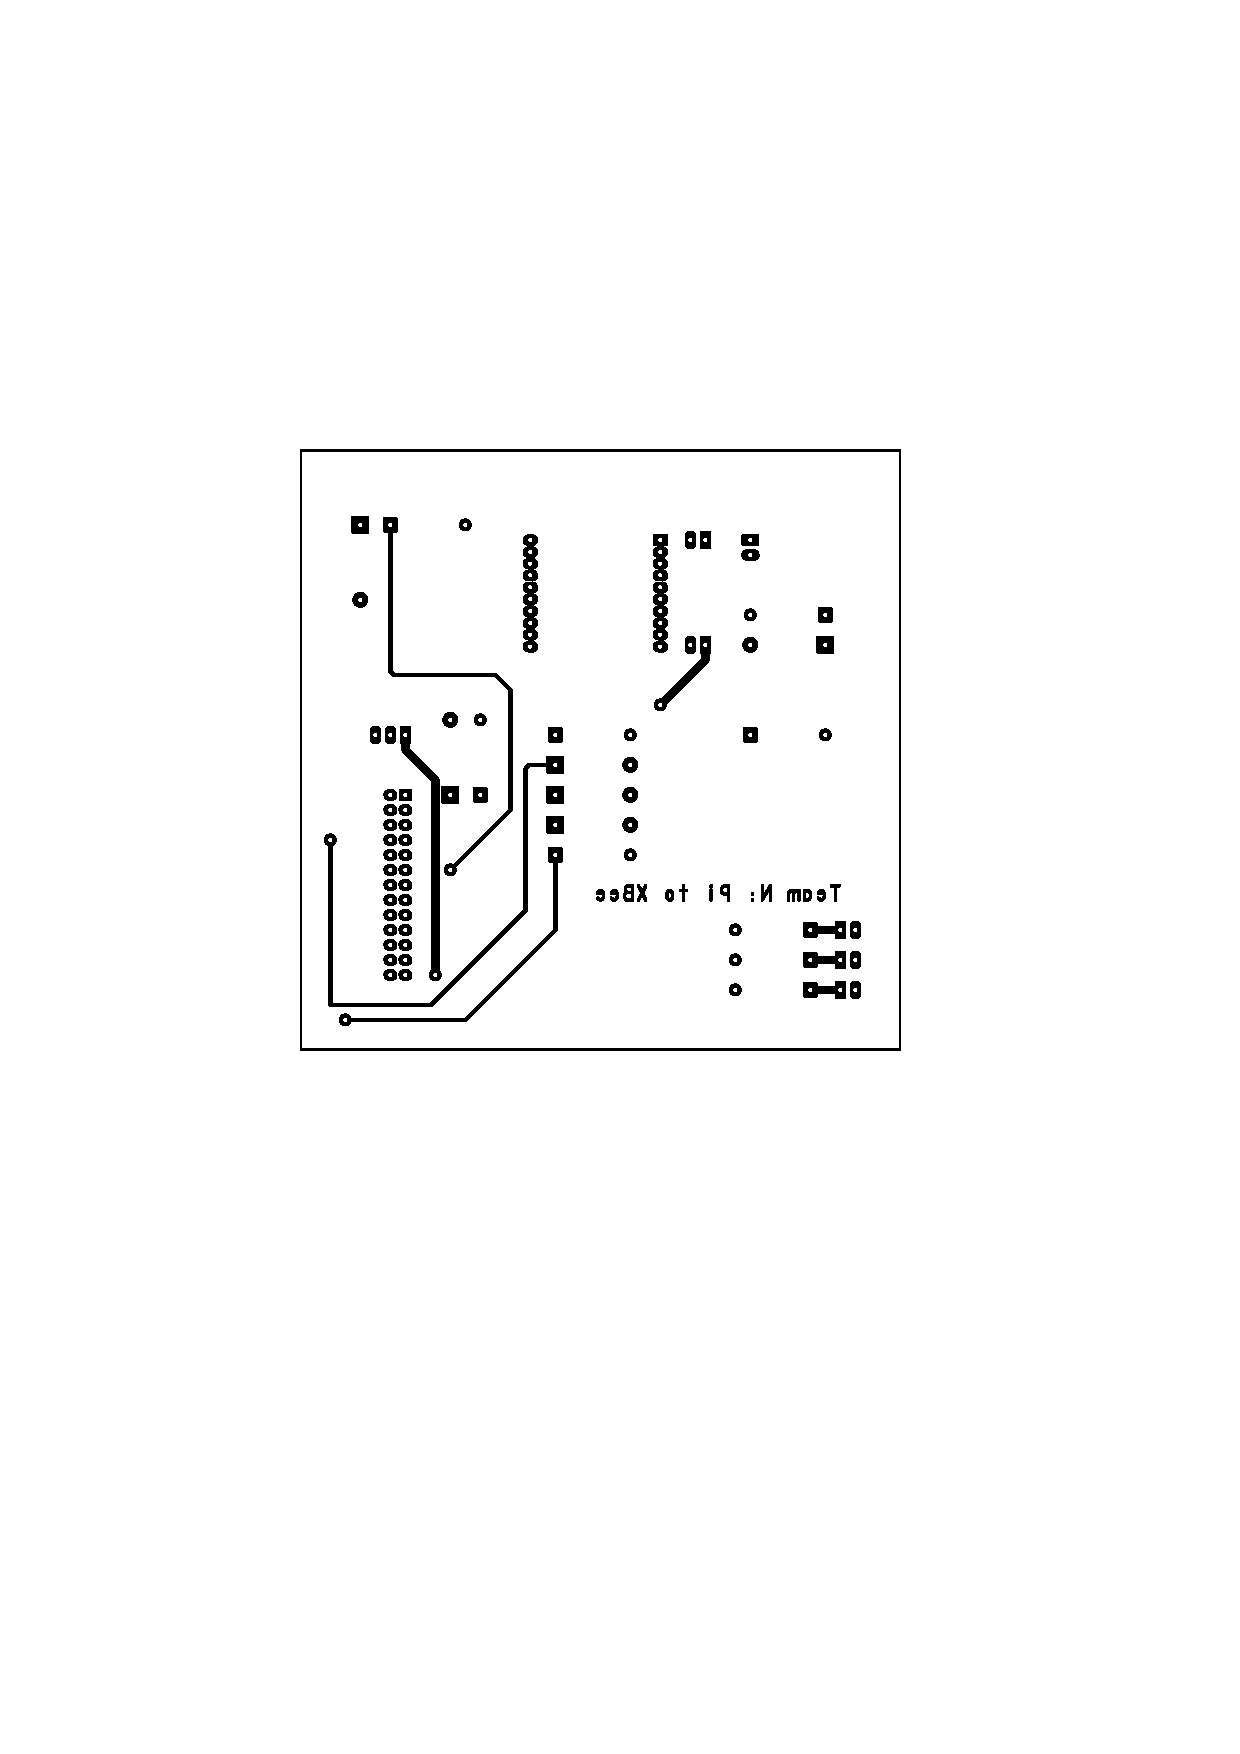
\includegraphics[scale=0.6]{figures/Pi2XBee_top}
\end{center}
\caption{PCB Photomask: RaspberryPi to XBee - Top}
\label{fig:Pi2XBee3}
\end{figure}

\begin{figure}[H]
\begin{center}
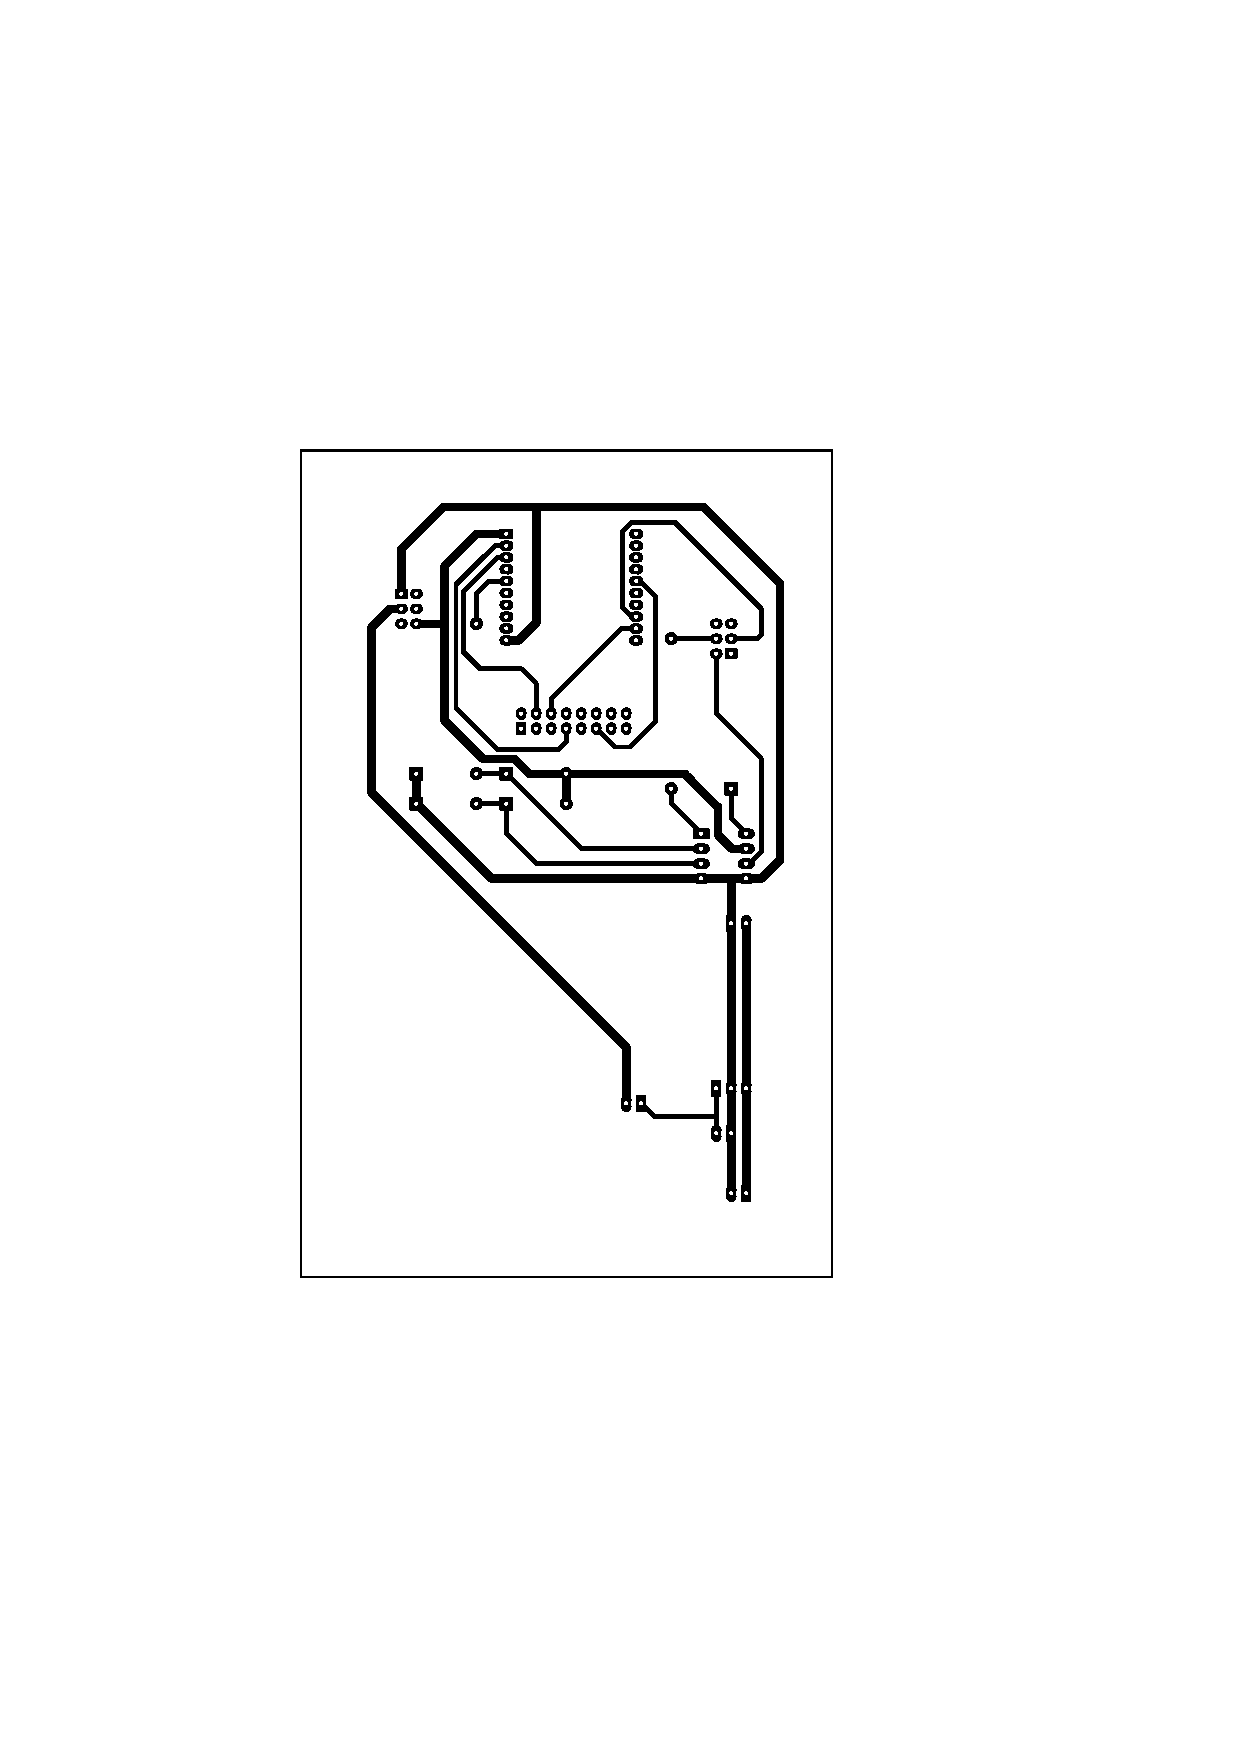
\includegraphics[scale=0.6]{figures/ARM2XBee_bottom}
\end{center}
\caption{PCB Photomask: ARM to XBee - Bottom}
\label{fig:ARM2XBee2}
\end{figure}

\begin{figure}[H]
\begin{center}
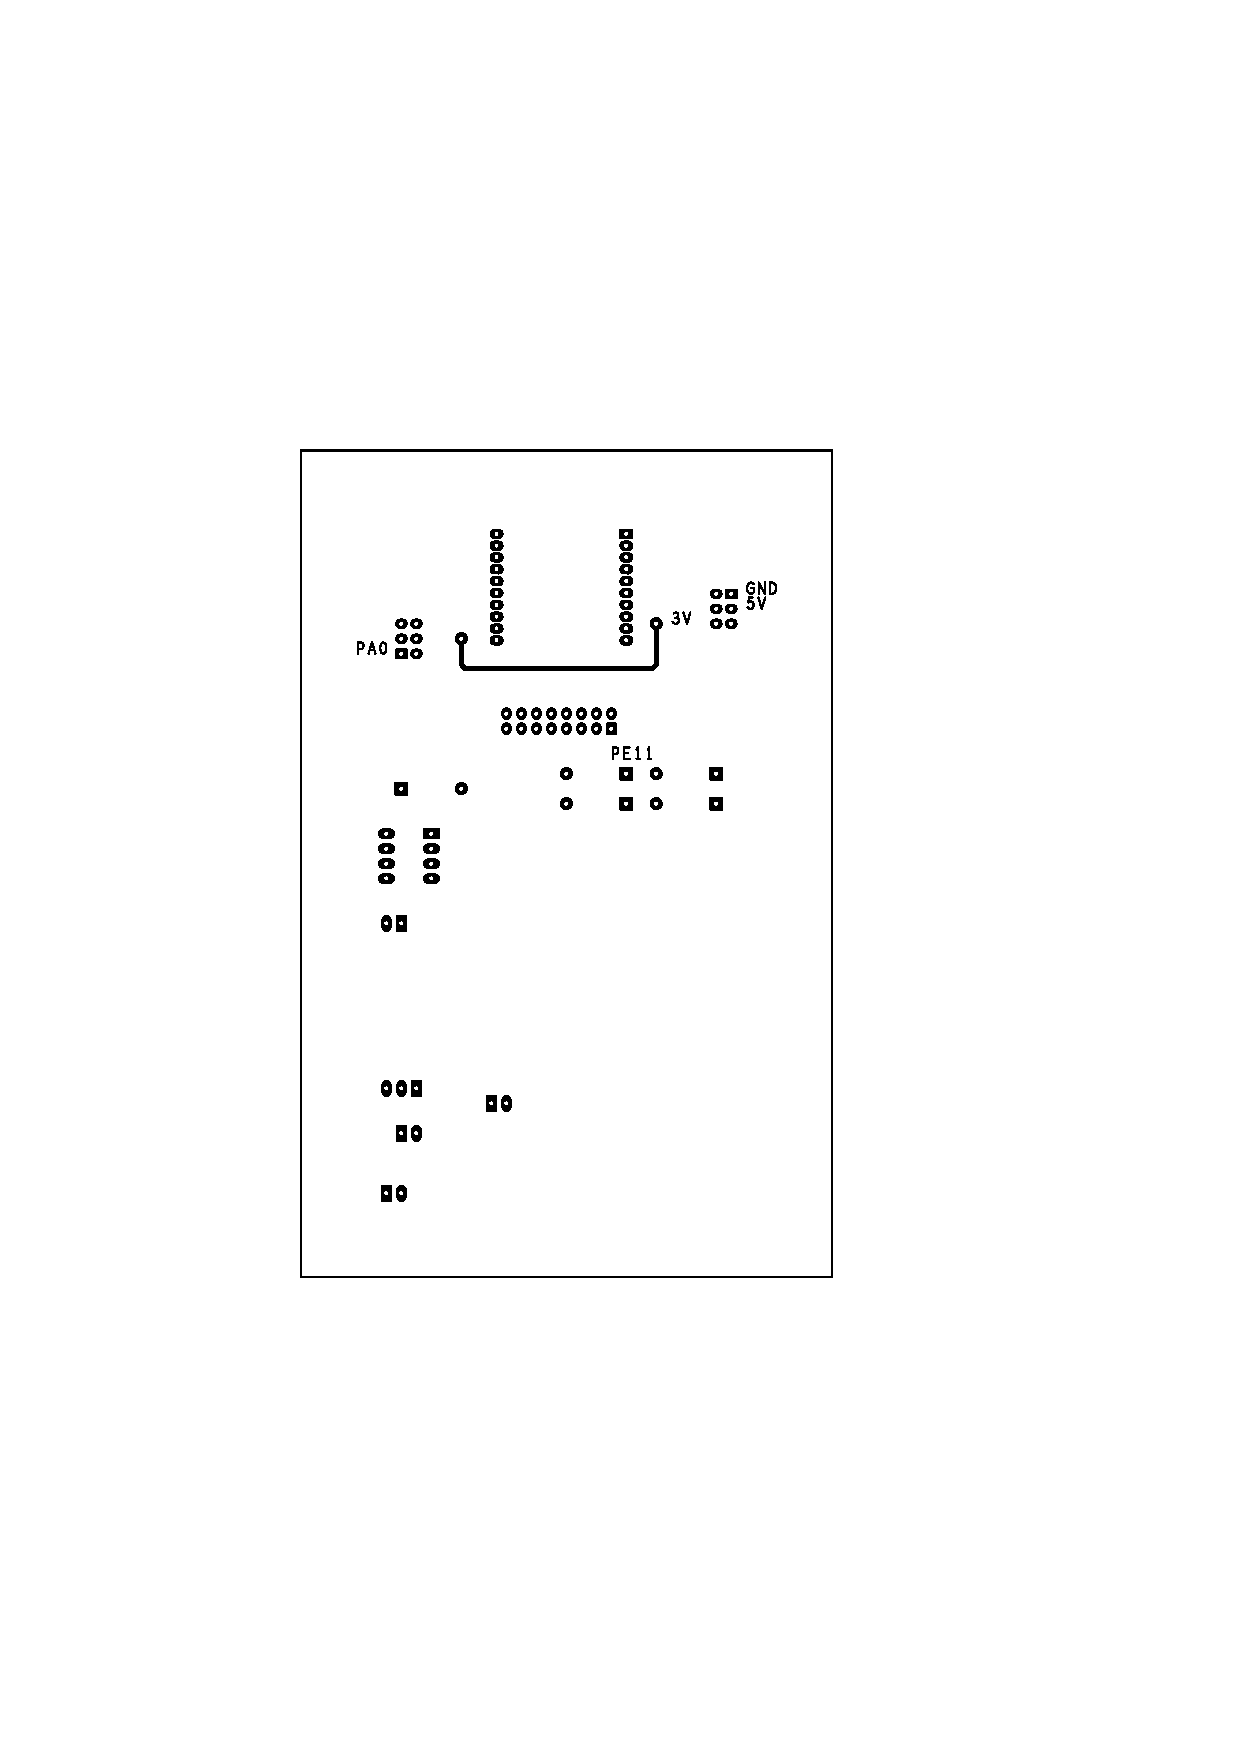
\includegraphics[scale=0.6]{figures/ARM2XBee_top}
\end{center}
\caption{PCB Photomask: ARM to XBee - Top}
\label{fig:ARM2XBee3}
\end{figure}

\end{document}
